\documentclass[10pt,aspectratio=43]{ISAE-Beamer}
\usefonttheme[onlymath]{serif}

% === PACKAGES === %

\usepackage{
amsmath,
amssymb,
amsthm,
dsfont,
%fontawesome,
multimedia,
tcolorbox,
ulem
}


\usetikzlibrary{arrows}
\usetikzlibrary{decorations.pathmorphing}
\usepackage{hyperref}

% ANDREA
%\usepackage{arydshln,mathtools}
%\usepackage{bm} %=>Fatal error occurred, no output PDF file produced!
% \usepackage[backend=bibtex,doi=false,isbn=false,url=false,eprint=false]{biblatex}
% Package biblatex Error: Incompatible package 'ucs'
% \bibliography{../mybibliography} %

%\bibliography{WavesPHSAnaNumNEW}

% === COLORS === %

\newcommand{\blue}[1]{\textcolor{blue}{#1}}
\colorlet{darkpurple}{purple!80!black}
\newcommand{\darkpurple}[1]{\textcolor{darkpurple}{#1}}
\colorlet{darkgreen}{green!50!black}
\newcommand{\green}[1]{\textcolor{darkgreen}{#1}}
\colorlet{darkorange}{orange!90!black}
\newcommand{\orange}[1]{\textcolor{darkorange}{#1}}
\newcommand{\purple}[1]{\textcolor{purple}{#1}}
\newcommand{\red}[1]{\textcolor{red}{#1}}

% === MACROS === %

% = A = %
\newcommand{\Alpha}{\vector{\alph}}
\newcommand{\alphap}{\alph_p}
\newcommand{\Alphaq}{\Alpha_q}
\newcommand{\Alphav}{\boldsymbol{\alpha}_v}
\newcommand{\alp}{\vector{\alph}}
\renewcommand{\alph}{\purple{\alpha}}



% = B = %
\newcommand{\biblio}{\blue{\tiny\faBook}}

\newcommand{\bm}{\boldsymbol} 
% = C = %
\renewcommand{\check}{\red{\checkmark}}
\newcommand{\curl}{\vector{\rm curl}}

% = D = %
\newcommand{\D}{\green{\mc D}}
\newcommand{\dd}{{\rm ~d}}
\renewcommand{\div}{{\rm div}}
\newcommand{\divs}{{\mbox{\rm \tiny div}}}
\newcommand{\dsp}{\displaystyle}
\DeclareMathOperator*{\Div}{Div}
% = E = %
\newcommand{\E}{\purple{\mc E}}
\newcommand{\Eo}{\orange{E}}
\newcommand{\e}{\vector{\eff}}
\newcommand{\eff}{\purple{e}}
\newcommand{\eg}{\textit{e.g.~}}
\renewcommand{\emph}{\textbf}
\newcommand{\epso}{\orange{\epsilon}}
\newcommand{\eqdef}{:=}

\newcommand{\energy}[1]{\frac{1}{2} \int_{\Omega} \left\{ #1 \right\} \dd\Omega}

% = F = %
\newcommand{\F}{\darkpurple{\mc F}}
\newcommand{\f}{\darkpurple{\vector{f}}}
\newcommand{\flo}{\darkpurple{f}}
\newcommand{\Forall}{ \quad \forall }

% = G = %
\newcommand{\grad}{\vector{\rm grad}}
\newcommand{\graph}{\mbox{\rm Graph}}
\DeclareMathOperator*{\Grad}{Grad}

% = H = %
\renewcommand{\H}{\mathbf{H}}
\newcommand{\Ham}{\green{\mc H}}
\DeclareMathOperator*{\Hess}{Hess}

% = I = %
\newcommand{\idea}{\raisebox{-0.1cm}{\textcolor{yellow!80!red}{\LARGE\faLightbulbO}}~}
\newcommand{\ie}{\textit{i.e.~}}
\newcommand{\inner}[3][]{\ensuremath{\left\langle #2, \, #3 \right\rangle_{#1}}}


% = J = %
\newcommand{\J}{\green{\mc J}}

% = K = %

% = L = %
\renewcommand{\L}{\mathbf{L}}
\newcommand{\LambdaTens}{\orange{\overline{\overline{\boldsymbol \lambda}}}}

% = M = %
\newcommand{\matl}{\left(\begin{matrix}}
\newcommand{\matr}{\end{matrix}\right)}
\newcommand{\mc}{\mathcal }

% = N = %
\newcommand{\n}{\vector{n}}
\newcommand{\nuo}{\blue{{\boldsymbol \nu}}}
\newcommand{\nol}{\left\Vert}
\newcommand{\nor}{\right\Vert}
\newcommand*{\norm}[1]{\ensuremath{\left\|#1\right\|}}

% = O = %
\newcommand{\one}{\mathds{1}}

% = P = %
\renewcommand{\P}{\mathbb{P}}
\newcommand{\pbl}{\left[}
\newcommand{\pbr}{\right]}
\newcommand{\psl}{\left\langle}
\newcommand{\psr}{\right\rangle}

% = Q = %

% = R = %
\newcommand{\R}{\mathbb{R}}
\newcommand{\rhoo}{\orange{\rho}}

% = S = %
\newcommand{\s}{\vector{s}}
\renewcommand{\S}{\green{\mc S}}

% = T = %
\newcommand{\Tens}{\orange{\overline{\overline{\boldsymbol T}}}}

% = U = %
\renewcommand{\u}{\blue{{\boldsymbol u}}}
\newcommand{\uv}{\blue{\vector{u}}}
\newcommand{\U}{\green{\mc U}}

% = V = %
\renewcommand{\v}{\vector{v}}
\renewcommand{\vector}[1]{\overrightarrow{\mathbf{\boldsymbol #1}}}

% = W = %
\newcommand{\warning}{\red{\faWarning}~}

% = X = %
\newcommand{\x}{\vector{x}}

% = Y = %
\newcommand{\y}{\red{{\boldsymbol y}}}
\newcommand{\yv}{\red{\vector{y}}}

% = Z = %
\newcommand{\Zo}{\orange{Z}}

% === TITLE INFORMATIONS === %

\title[PFEM 4 PHS]{\blue{Numerics for PH-PDEs}:\\
  \vspace{2mm}
  the Partitioned Finite Element Method,\\
  \vspace{2mm}
a structure-preserving method for physics-based PDEs with boundary control.}

 %The Partitioned Finite Element Method for port-Hamiltonian systems: structure-preserving numerics for physics-based PDEs\\ with boundary control}

\institute[ISAE-SUPAERO]{	\inst{1} ISAE-SUPAERO, Universit\'e de Toulouse}

\author[D. Matignon]{\texorpdfstring{Denis Matignon\inst{1}}{Denis Matignon}}

\date[2nd Spring School on Theory \& Applications of pHs]{\texorpdfstring{\textit{2nd Spring School on Theory \& Applications of pHs}\\ 25th March 2022, FrauenInsel}{Thematic Einstein Semester, 14 th January 2021, Berlin}}

\thanks{\texorpdfstring{\includegraphics[scale=0.11]{~/Documents/INFIDHEM/PHS2021WIAS/Figures/INFIDHEM-logo}}{INFIDHEM}}

\begin{document}

\maketitle

\begin{frame}{Outline}

\tableofcontents

\end{frame}

%%%%%%%%%%%%%%%%%%%%%%%%%%%%%%%%%%%
%%% INTRO
%%%%%%%%%%%%%%%%%%%%%%%%

%%%%%%%%%%%%%%%%%ùù
\iffalse
\begin{frame}
  Bonjour
  
  $\boldsymbol{\alpha}$, $\bm{\alpha}$
  
 $\phi$  ${\boldsymbol \phi}$ $\boldsymbol{\phi}$, $\bm{\phi}$ $\int_\Omega  {\bm{\phi}}_h\cdot{\bm{\phi}}_h^\top$

  $\boldsymbol{\Phi}$, $\bm{\Phi}$ $\int_\Omega  {\bm{\Phi}}_v\cdot{\bm{\Phi}}_v^\top$
\end{frame}
\fi


%%%%%%%%%%%%%%%% INTRO GENERALE
\section{Introduction}

%%%%%%%%%%%%%%%%%%%% SS  GOAL
\subsection{Goal of the presentation}
\begin{frame}
  \begin{itemize}

  \item Make links with other courses given at this Spring School:
    \begin{enumerate}
    \item \blue{course on infinite-dimensional PH-PDEs by Birgit Jacob and Hans Zwart},
    \item \blue{course on PH-DAEs by Volker Mehrmann and Arjan van der Schaft},
      \item \blue{course on Thermodynamics by Hans-Christian {\"O}ttinger}.
\end{enumerate}
    % Links with the course Hans and Birgit on PH-PDEs, wiht the course of Volker on PH-DAEs, and with the course of Hans-Christian on Thermodynamics

  \item {\bf Main Goal}: the underlying structure of physical systems must be preserved by numerical methods at the discrete level, i.e. from infinite dimension to finite dimension (but still in continuous time).

  \item The question of \blue{specific time discretization addressed in the course by Paul Kotyczka and Laurent Lefèvre}, just before, will not be tackled in the sequel.
  \end{itemize}
\end{frame}

%%%%%%%%%%%%%%%%%%%% SS REFERENCES
\subsection{A few references}

\begin{frame}
  \frametitle{\small A recent reference on distributed port-Hamiltonian systems}
\idea \blue{Twenty years of distributed port-Hamiltonian systems: a literature review}

\textbf{\quad Rashad, R.,  Califano, F.,  van der Schaft, A.J. and Stramigioli, S.}

\quad \textit{IMA J. Mathematics of Control and Information, \\
  \quad vol.37 (4), pp. 1400--1422 (2020)}

\vspace{5mm}

$\Longrightarrow$ More than 170 up-to-date references on:
\begin{itemize}
\item Theoretical Framework
\item Modeling
\item Analysis and Control
\item \underline{Discretization}
  \end{itemize}
\end{frame}

\begin{frame}{and more specifically}
  \begin{itemize}
  \item \blue{Numerical Methods for Distributed Parameter Port-Hamiltonian Systems}
    \textbf{\quad Kotyczka P.}
     \quad  \textit{TUM University Press, Munich (2019)},
  \item \blue{Structure preserving approximation of dissipative evolution problems}
    \textbf{\quad  Egger H.}
    \quad  \textit{Numerische Mathematik vol.143(1), pp. 85--106 (2019)}
    \item \blue{A Partitioned Finite-Element Method for power-preserving discretization of open systems of conservation laws},
\textbf{\quad Cardoso-Ribeiro F.L., Matignon D., Lef\`evre L.}
\quad  \textit{IMA J. Mathematics of Control and Information, vol.38(2), pp. 493--533 (2021)}
\item \blue{Numerical Approximation of Port-Hamiltonian
Systems for Hyperbolic or Parabolic PDEs with
Boundary Control},
  \textbf{\quad Brugnoli A., Haine G., Serhani A., Vasseur X.}
  \quad  \textit{Journal of Applied Mathematics and Physics, vol.9,  pp. 1278--1321 (2021)}.
    \end{itemize}

  \end{frame}


%%%%%%%%%%%%%%%%%%%% SS  OBJECTIVE
\subsection{Main objective of PFEM}

\begin{frame}
\frametitle{Main Objective}
\onslide<1->\begin{block}{Aim:}
\textit{\green{Simulate}} \textit{\blue{complex open physical systems}} by ensuring the \textit{\red{conservation of the \emph{\underline{power balance}}}} for a chosen functional: the \emph{Hamiltonian}.
\end{block}\vfill

\begin{itemize}
\item<2->
\green{\underline{\textit{Finite Element Method:}}}

$\rightarrow$ \emph{Complex geometries} are allowed.

$\rightarrow$ A wide range of \emph{implementation} tools are available.\vfill

\item<3->
\blue{\underline{\textit{Port-Hamiltonian Systems (PHS):}}}

$\rightarrow$ Model \emph{``energy'' exchanges} between simpler open subsystems.

$\rightarrow$ The power balance is \textit{encoded} in a \emph{Stokes-Dirac structure}.\vfill

\item<4->
\red{\underline{\textit{Partitioned Finite Element Method (PFEM):}}}

$\rightarrow$ It approximates the Stokes-Dirac structure into a \emph{Dirac structure}.

$\rightarrow$ The \emph{discrete Hamiltonian} satisfies a ``discrete'' power balance.
\end{itemize}
\vfill
\onslide<4->{\small
\idea \blue{A Partitioned Finite-Element Method for power-preserving discretization of open systems of conservation laws}

\textbf{\quad Cardoso-Ribeiro F.L., Matignon D., Lef\`evre L.}

\quad  \textit{IMA J. Mathematics of Control and Information, vol.38(2) , pp. 493--533 (2021)}
}
\end{frame}

\begin{frame}{Change of paradigm?}

\begin{center}
\begin{tikzpicture}[scale=1]
\onslide<1->
\draw (-3,0) node{``Context and Axioms''} ellipse (2cm and 1cm); 
\node[rotate=8] at (-3.75,0.5) {\tiny Conservation of mass};
\node[rotate=-5] at (-1.8,0.4) {\tiny Rigid body};
\node[rotate=-6] at (-3.5,-0.65) {\tiny Constant temperature};
\draw (0,0) node{\green{${\boldsymbol \&}$}};
\draw (0,-0.25)  node[below]{\uwave{Energy} $\Ham$}; 
\draw (3,0) node{``Definitions and Laws''} ellipse (2cm and 1cm); 
\node[rotate=-8] at (3.75,0.5) {\tiny $p \eqdef mv$};
\node[rotate=5] at (1.8,0.4) {\tiny Fourier's law};
\node[rotate=6] at (3.5,-0.65) {\tiny Hooke's law};
\draw[darkgreen,very thick,dashed] (-5.25,-1.75) -- (6,-1.75);
\draw[darkgreen,very thick,dashed] (-5.25,-3.9) -- (6,-3.9);
\draw[decorate,decoration=snake,very thick] (0,-1.5) -- (0,-7); 
\draw[darkgreen] (-5.25,0) node{\rotatebox{90}{\textbf{Physics}}};
\draw[darkgreen] (-5.25,-2.85) node{\rotatebox{90}{\textbf{Modelling}}};
\draw[darkgreen] (-5.25,-5.3) node{\rotatebox{90}{\textbf{Discretization}}};

\onslide<2->
\draw (-3,-3) node{\emph{PDE}} ellipse (1cm and 0.5cm); 
\draw[red,thick] (-2.5,-0.5) -- (-2,-1.5); 
\draw[->,red,thick] (-2,-1.5) -- (-3,-2.75); 
\draw[red,thick] (2.5,-0.5) -- (-2,-1.5); 
\draw[white,fill=white] (-2,-1.5) node{$\red{\oplus}$} circle (0.125cm); 
\draw[->,red,thick] (-3,-3.25) -- (-3,-5.5); 
\draw[red] (-3,-4.75) node{\textbf{FEM}}; 
\draw (-3,-5.75) node{\; \; Well-proven \& Robust \check}; 
\draw (-3,-6.25) node{\; \; How does $\Ham_d$ evolve\red{?}}; 
\draw (-3,-6.75) node{\; \; Control\red{?} \quad Coupling\red{?}}; 
\draw (-2.5,-0.5) node{$\bullet$}; 
\draw (2.5,-0.5) node{$\bullet$}; 

\onslide<3->
\node at (1.5,-2.2) {\red{Structure}};
\draw (1.5,-3) node{\emph{PHDAE}} ellipse (1cm and 0.5cm); 
\draw[blue] (3,-3) node{${\boldsymbol \&}$}; 
\node at (4.5,-2.2) {\red{Closure}};
\draw (4.5,-3) node{\emph{Cons. Rel.}} ellipse (1cm and 0.5cm); 
\draw[->,blue,thick] (-2.5,-0.5) -- (1.5,-2.75); 
\draw[->,blue,thick] (2.5,-0.5) -- (4.5,-2.75); 
\draw[->,blue,thick] (1.5,-3.25) -- (1.5,-5.5); 
\draw[->,blue,thick] (4.5,-3.25) -- (4.5,-5.5); 
\draw[blue] (3,-4.75) node{\textbf{PFEM}}; 
\draw (3,-5.75) node{\; \; Known $\Ham_d$ \check \; $\blue{\boldsymbol \&}$ \; DAE \warning}; 
\draw (3,-6.25) node{\; Designed for control \check}; 
\draw (3,-6.75) node{\; Well-suited for coupling \check}; 

\onslide<1->
\end{tikzpicture}
\end{center}
\end{frame}

%\subsection{Definitions and Notations}
\begin{frame}{Port-Hamiltonian Systems (PHS)}

\begin{itemize}
\item<1->
The \emph{energy variables} $\alp$ (vector field);
\item<1->
The \emph{Hamiltonian} $\Ham(\alp(t))$ (positive functional);
\item<2->
The \emph{co-energy variables} $\e_{\alp} \eqdef \delta_{\alp} \Ham$ (vector field), \\ \qquad $\leadsto$ the variational derivative of $\Ham$ w.r.t $\alp$;
\item<3->
The \emph{\textit{structure} operator} $J$ (linear and \textit{formally skew-symmetric});
\item<3->
The \emph{resistive/dissipative operator} $R$ (linear and \textit{positive});
\item<4->
The \emph{control operator} $B$ (linear);
\item<4->
The \emph{input} $\u$ and the \emph{collocated output} $\y$ (boundary fields);
\item<5->
The \emph{dynamical system}:
\begin{tcolorbox}
\centering
$
\left\{\begin{array}{l}
\partial_t \alp(t) = \left( J - R \right) \e_{\alp}(t) + B \u(t), \\
\y(t) = B^* \e_{\alp}(t).
\end{array}\right.
$
\end{tcolorbox}
\end{itemize}
\onslide<6->
\begin{alertblock}{\textbf{Lossy Power Balance}}
\centering
$
\frac{\rm d}{{\rm d}t} \Ham(\alp(t)) = - \psl R \e_{\alp}(t), \e_{\alp}(t) \psr_J + \psl \u(t), \y(t) \psr_B \; \le \; \psl \u(t), \y(t) \psr_B.
$
\end{alertblock}
\hspace{-6pt}\warning\hspace{-6pt} Although \textbf{\red{the underlying geometry}} is well-determined with the above equality, \emph{constitutive relations} between $\alp$ and $\e_{\alp}$ are also needed to solve the system!

\end{frame}


%%%%%%%%%%%%%%%%%%%%%%%%%%%%%%%%%%%%%%%
%%%%%%%%%%%%%%%% LINEAR %%%%%%%%%%%%%%
%%%%%%%%%%%%%%%%%%%%%%%%%%%%%%%%%%%%%%%
 \section{Linear Wave equations: towards PH-DAEs and PH-ODEs}

 %%%%%%%%%%%%%%%%%%%% SS Discretieaion PH DAEs
\subsection{Discretization in terms of energy and co-energy variables: PH-DAEs}

\begin{frame}{Conservative System: Wave as PH-DAE}

\onslide<1-> \textbf{\red{Deflection} $w$ of a 2D-membrane, \blue{\textit{boundary deflection velocity} as control}.}\vfill
\onslide<2-> Its total energy is given by the sum of the potential \& kinetic energies:\vfill
\centering
$
\dsp \Ham(\alp_q, \alph_p) 
\eqdef \frac{1}{2} \int_\Omega \left( \alp_q \cdot \Tens \cdot \alp_q + \frac{1}{\rhoo} \alph_p^2 \right).
$
\begin{itemize}
\item<3->
$\rhoo$ the \textit{mass density} of the medium and $\Tens$ the \textit{Young modulus} tensor;
\item<3->
$\alph_p \eqdef \rhoo\,\partial_t w$ the \textit{linear momentum} and $\alp_q \eqdef \grad \left( w \right)$ the \textit{strain};
\item<4->
$\e_q \eqdef \delta_{\alp_q} \Ham = \Tens \cdot \alp_q$ the \textit{stress};
\item<4->
$\eff_p \eqdef \delta_{\alph_p} \Ham = \frac{\alph_p}{\rhoo} = \partial_t w$ the \blue{\it deflection velocity} and $\u \eqdef \eff_p$;
\item<5->
$\y \eqdef \e_q \cdot \n$ the output \red{\it normal stress}.
\end{itemize}
\onslide<6->
{\small
$$
\left\{\begin{array}{rl}
\rhoo \partial_{tt}^2 w &= \div \left( \Tens \cdot \grad \left( w \right) \right), \\
\u &= \partial_t w, \\
\y &= \left( \Tens \cdot \grad \left( w \right) \right) \cdot \n.
\end{array}\right.
\onslide<7->
\hspace{-10pt}
\Leftrightarrow
\hspace{-2pt}
\left\{\begin{array}{rl}
\partial_t \alp_q &= \grad \left( \eff_p \right), \\
\partial_t \alph_p &= \div \left( \e_q \right),
\end{array}\right.
\hfill
\&
\hfill
\left\{\begin{array}{rl}
\u &= \eff_p, \\
\y &= \e_q \cdot \n.
\end{array}\right.
$$}
\onslide<8->
\begin{alertblock}{Lossless \textbf{Power Balance}}
\centering
$
\frac{\rm d}{{\rm d}t}\Ham (\alp_q, \alph_p) 
= \psl \y, \u \psr_{H^{-\frac{1}{2}},H^{\frac{1}{2}}}.
$
\end{alertblock}

$\Longrightarrow$  for infinite-dimensional pHs in general,  \blue{see the course by Birgit Jacob and Hans Zwart on Wednesday morning}.
\end{frame}

\begin{frame}{Conservative System: PFEM strategy}

\onslide<1->
\begin{block}{The strategy follows:}
\begin{enumerate}
\item<2->
Write the \textbf{weak formulation};
\item<3->
Apply an accurate \textbf{Stokes (Green) identity} (such that $\u$ ``appears'');
\item<4->
Project on a finite-dimensional space thanks to \textbf{FEM}.
\end{enumerate}
\end{block}
\vfill
\onslide<5-> For all test functions $\v_q$, $v_p$ and $v_\partial$ (smooth enough):
$$
~\hspace{-0.5cm}\left\{\begin{array}{l}
\dsp \psl \partial_t \alp_q, \v_q \psr_{\L^2} = \psl \grad \left( \eff_p \right), \v_q \psr_{\L^2}, \\
\dsp \psl \partial_t \alph_p, v_p \psr_{L^2} = \psl \div \left( \e_q \right), v_p \psr_{L^2}, \\
\dsp \psl \y, v_\partial \psr_{H^{-\frac{1}{2}},H^{\frac{1}{2}}} = \psl \e_q \cdot \n, v_\partial \psr_{H^{-\frac{1}{2}},H^{\frac{1}{2}}}.
\end{array}\right.
$$
\onslide<6-> Applying Green's formula on the 1st line and using the definition of $\u$:
$$
\psl \partial_t \alp_q, \v_q \psr_{\L^2} = - \psl \eff_p, \div \left( \v_q \right) \psr_{L^2} 
+ \psl \v_q \cdot \n, \u \psr_{H^{-\frac{1}{2}},H^{\frac{1}{2}}}.
$$
\vfill
\onslide<7-> 
\begin{tcolorbox}
Green's formula applied on the 2nd line would lead to normal stress control $\u = \e_q \cdot \n$. The energy variables are \textbf{partitioned} accordingly.
\end{tcolorbox}

\end{frame}

\begin{frame}{Conservative System: FEM Application}

The energy, co-energy, boundary and test functions of the \textit{same} index are discretized by using the \textit{same} bases, either scalar- or \textbf{vector}-valued:
$$
\begin{array}{ll}
\onslide<1-> \alp_q^{ap}(t,\x) \eqdef \sum_{\ell=1}^{N_q} \vector{\phi}_q^\ell(\x) \alph_q^\ell(t) = \vector{\Phi}_q^\top \cdot \underline{\alph}_q(t), &
\onslide<2-> \e_q^{ap}(t,\x) =  \vector{\Phi}_q^\top \cdot \underline{\eff}_q(t), \\
\onslide<3->\alph_p^{ap}(t,\x) \eqdef \sum_{k=1}^{N_p} \varphi_p^k(\x) \alph_p^k(t) = {\boldsymbol \phi}_p^\top \cdot \underline{\alph}_p(t), &
\eff_p^{ap}(t,\x) = {\boldsymbol \phi}_p^\top \cdot \underline{\eff}_p(t), \\
\onslide<4->\u^{ap}(t,\s) \eqdef \sum_{m=1}^{N_{\partial}} \psi^m(\s) \u^m(t) = {\boldsymbol \Psi}^\top \cdot \underline{\u}(t), & 
\y^{ap}(t,\s) = {\boldsymbol \Psi}^\top \cdot \underline{\y}(t),
\end{array}
$$
\onslide<1-> with $\vector{\Phi}_q$ an $N_q \times 2$ matrix, \onslide<3-> ${\boldsymbol \phi}_p$ an $N_p \times 1$ matrix \onslide<4-> and ${\boldsymbol \Psi}$ an $N_{\partial} \times 1$ matrix.\vfill
\onslide<5->
\begin{block}{The discretized system (giving the structure) then reads:}
\centering
$
\left\{\begin{array}{l}
\vector{M}_q \cdot \frac{\rm d}{{\rm d}t}\underline{\alph}_q(t) = D \cdot \underline{\eff}_p(t) + B \cdot \underline{\u}(t), \\
M_p \cdot \frac{\rm d}{{\rm d}t}\underline{\alph}_p(t) = -D^\top \cdot \underline{\eff}_q(t), \\
M_\partial \cdot \underline{\y}(t) = B^\top \cdot \underline{\eff}_q(t),
\end{array}\right.
$
\end{block}
\flushleft\onslide<6-> where:
$$
\begin{array}{c}
\vector{M}_q \eqdef \int_\Omega \vector{\Phi}_q \cdot \vector{\Phi}_q^\top, \qquad
M_p \eqdef \int_\Omega {\boldsymbol \phi}_p \cdot {\boldsymbol \phi}_p^\top, \qquad
M_\partial \eqdef \int_{\partial\Omega} {\boldsymbol \Psi} \cdot {\boldsymbol \Psi}^\top, \\
~ \\
D \eqdef - \int_\Omega \div\left( \vector{\Phi}_q \right) \cdot {\boldsymbol \phi}_p^\top, \qquad
B \eqdef \int_{\partial\Omega} \left( \vector{\Phi}_q \cdot \n \right) \cdot {\boldsymbol \Psi}^\top.
\end{array}
$$
\end{frame}

\begin{frame}{Conservative System: Power Balance}

\onslide<1->
\begin{alertblock}{Finite-Dimensional extended structure operator}
\centering
$
\green{\J}_d \eqdef \matl 0 & D & B \\ -D^\top & 0 & 0 \\ -B^\top & 0 & 0 \matr.% \quad \Longrightarrow \quad \D_d \eqdef \graph \left( \green{\J}_d \right).
$
\end{alertblock}
\onslide<2-> \warning The inner product on $\R^{N_q}$, $\R^{N_p}$ and $\R^{N_\partial}$ has to be taken w.r.t. the mass matrices $\vector{M}_q$, $M_p$ and $M_\partial$: \eg $\psl \v_1, \v_2 \psr_{N_q} \eqdef \v_2^\top \cdot \vector{M}_q \cdot \v_1$.\vspace{-2pt}
\onslide<3-> 
\begin{alertblock}{Discrete Hamiltonian}
\centering
$
\green{\Ham}_d \left( \underline{\alph}_q, \underline{\alph}_p \right) \eqdef \Ham \left( \alp_q^{ap}, \alph_p^{ap} \right) = \frac{1}{2} \left( \underline{\alph}_q^\top \cdot \vector{M}_{\Tens} \cdot \underline{\alph}_q + \underline{\alph}_p^\top \cdot M_{\frac{1}{\rhoo}} \cdot \underline{\alph}_p \right),
$\vfill
\onslide<4-> $\vector{M}_{\Tens} \eqdef \int_\Omega \vector{\Phi}_q \cdot \Tens \cdot \vector{\Phi}_q^\top$ \qquad \& \qquad $M_{\frac{1}{\rhoo}} \eqdef \int_\Omega \frac{1}{\rhoo} {\boldsymbol \phi}_p \cdot {\boldsymbol \phi}_p^\top$.
\end{alertblock}
\onslide<5-> \textbf{Constitutive relations}: \quad $\vector{M}_q \cdot \underline{\eff}_q = \vector{M}_{\Tens} \cdot \underline{\alph}_q$ \quad \& \quad $M_p \cdot \underline{\eff}_p = M_{\frac{1}{\rhoo}} \cdot \underline{\alph}_p$ \hfill \check \check \vfill
\onslide<6-> Denote $\underline{\flo} \eqdef \matl \frac{\rm d}{{\rm d}t}\underline{\alph}_q, & \frac{\rm d}{{\rm d}t}\underline{\alph}_p, & -\underline{\y} \matr^\top$ and $\underline{\eff} \eqdef \matl \underline{\eff}_q, & \underline{\eff}_p, & \underline{\u} \matr^\top$, then:
\begin{alertblock}{Discrete Lossless \textbf{Power Balance}}
\centering
$
%\matl \underline{\flo} \\ \underline{\eff} \matr \in \D_d \; \Rightarrow \; \psl \underline{\flo}, \underline{\eff} \psr_{N_p, N_q, N_\partial} = 0 
%\; \Rightarrow \; 
\frac{\rm d}{{\rm d}t}\Ham_d \left( \underline{\alph}_q, \underline{\alph}_p \right) = \underline{\u}^\top \cdot M_\partial \cdot \underline{\y}.
$
\end{alertblock}

\end{frame}


\begin{frame}{A Proof of the Discrete Power Balance}
  Since by definition the discrete Hamiltonian reads:
  $$\green{\Ham}_d \left( \underline{\alph}_q, \underline{\alph}_p \right)  = \frac{1}{2} \left( \underline{\alph}_q^\top \cdot \vector{M}_{\Tens} \cdot \underline{\alph}_q + \underline{\alph}_p^\top \cdot M_{\frac{1}{\rhoo}} \cdot \underline{\alph}_p \right),$$
  we can compute its time derivative along the trajectories:
  \begin{eqnarray*}
    \frac{\rm d}{{\rm d}t}\Ham_d \left( \underline{\alph}_q, \underline{\alph}_p \right)
    &=& ({\frac{\rm d}{{\rm d}t}\underline{\alph}_q})^\top \cdot \vector{M}_{\Tens} \cdot \underline{\alph}_q + ({\frac{\rm d}{{\rm d}t}\underline{\alph}_p})^\top \cdot M_{\frac{1}{\rhoo}} \cdot \underline{\alph}_p ,\\
    &=& ({\frac{\rm d}{{\rm d}t}\underline{\alph}_q})^\top \cdot \vector{M}_q \cdot \underline{\eff}_q + ({\frac{\rm d}{{\rm d}t}\underline{\alph}_p})^\top \cdot M_p \cdot \underline{\eff}_p ,\\
    &=& (\vector{M}_q\cdot {\frac{\rm d}{{\rm d}t}\underline{\alph}_q})^\top \cdot  \underline{\eff}_q + (M_p \cdot {\frac{\rm d}{{\rm d}t}\underline{\alph}_p})^\top \cdot \underline{\eff}_p ,\\
    &=& (  D \cdot \underline{\eff}_p(t) + B \cdot \underline{\u}(t) )^\top \cdot  \underline{\eff}_q + ( -D^\top \cdot \underline{\eff}_q(t)  )^\top \cdot \underline{\eff}_p ,\\
    &=&  \underline{\u}(t)^\top \cdot  B^\top\cdot  \underline{\eff}_q\\
    &=& \underline{\u}(t)^\top \cdot M_\partial \cdot\underline{\y}(t) . \qed
    \end{eqnarray*}
\end{frame}

\begin{frame}{PFEM for pHs gives rise to PH-DAEs}
  
  Summarizing the main steps: discretization of the structure and of the constitutive relations are made separately.
  
\begin{block}{The discretized system is a PH-DAE:}
\centering
$
\left\{\begin{array}{l}
\vector{M}_q \cdot \frac{\rm d}{{\rm d}t}\underline{\alph}_q(t) = D \cdot \underline{\eff}_p(t) + B \cdot \underline{\u}(t), \\
M_p \cdot \frac{\rm d}{{\rm d}t}\underline{\alph}_p(t) = -D^\top \cdot \underline{\eff}_q(t), \\
M_\partial \cdot \underline{\y}(t) = B^\top \cdot \underline{\eff}_q(t),
\end{array}\right.
$

together with

$
\left\{\begin{array}{l}
\vector{M}_q \cdot \underline{\eff}_q(t) = \vector{M}_{\Tens} \cdot \underline{\alph}_q(t), \\
M_p \cdot \underline{\eff}_p(t) = M_{\frac{1}{\rhoo}} \cdot \underline{\alph}_p(t)
\end{array}\right.
$
\end{block}


$\Longrightarrow$  in general, PFEM for pHs gives rise to finite-dimensional PH-DAEs, for which efficient numerical methods can be used (\blue{see the course by Volker Mehrmann on Tuesday morning})
  
\end{frame}


%%%%%%%%%%%%%%%%%%%%%%% SS Boundary Dissipation
\subsection{Application: Boundary Dissipation}


\begin{frame}{Impedance Boundary Condition (IBC)}

\onslide<1-> The Impedance Boundary Condition, with $\Zo\ge0$ on $\partial\Omega$, and $\nuo$ as new control, is considered:\hfill~
$
\nuo = \eff_p + \Zo \e_q \cdot \n
$\hfill~$\Leftrightarrow$\hfill~$\nuo = \partial_t w + \Zo \left( \Tens \cdot \grad \left( w \right) \right) \cdot \n$.~
\onslide<2-> \warning This kind of dissipation does not \textit{easily} fit in the ``$J-R$ framework''.\vfill
\onslide<3-> It can be seen as an \textit{output feedback law} $\u = -\Zo \y + \nuo$ in the previous case. 
\begin{alertblock}{Lossy \textbf{Power Balance}}
\centering
$
\frac{\rm d}{{\rm d}t}\Ham (\alp_q, \alph_p) 
= - \psl \y, \Zo \y \psr_{H^{-\frac{1}{2}},H^{\frac{1}{2}}} + \psl \y, \nuo \psr_{H^{-\frac{1}{2}},H^{\frac{1}{2}}}.
$
\vfill
\end{alertblock}
\vfill
\onslide<4-> Add \textbf{impedance ports} $(\flo_i, \eff_i)$ and \textbf{dissipative constitutive relation} $\eff_i = \Zo \flo_i$,\vfill
and approximate $\flo_i$ and $\eff_i$ in the boundary FEM basis ${\boldsymbol \Psi}$:
{\scriptsize~\vspace{-3pt}
$$
\matl
\vector{M}_q & 0 & 0 & 0 & 0 \\
0 & M_p & 0 & 0 & 0\\
0 & 0 & M_p & 0 & 0\\
0 & 0 & 0 & M_\partial & 0\\
0 & 0 & 0 & 0 & M_\partial 
\matr
\matl
\frac{\rm d}{{\rm d}t}\underline{\alph}_q(t) \\
\frac{\rm d}{{\rm d}t}\underline{\alph}_p(t) \\
\underline{\flo}_i(t) \\
- \underline{\y}(t) 
\matr
\hspace{-1.5pt}
=
\hspace{-1.5pt}
\matl
0 & D & -B & B \\
-D^\top & 0 & 0 & 0 \\
B^\top & 0 & 0 & 0 \\
-B^\top & 0 & 0 & 0 
\matr
\matl
\underline{\eff}_q(t) \\
\underline{\eff}_p(t) \\
\underline{\eff}_i(t) \\
\underline{\nuo}(t) 
\matr
$$}\vfill
and
\centering
$
M_\partial \cdot \underline{\eff}_i = \psl \Zo \psr \cdot \underline{\flo}_i, \qquad \qquad
$
with
$
\psl \Zo \psr \eqdef \int_{\partial\Omega} \Zo {\boldsymbol \Psi} \cdot {\boldsymbol \Psi}^\top \ge 0.
$
\onslide<5-> 
\begin{alertblock}{Discrete Lossy \textbf{Power Balance}}
\centering
$
\frac{\rm d}{{\rm d}t}\Ham_d \left( \underline{\alph}_q, \underline{\alph}_p \right) =  - \underline{\y}^\top \cdot \psl \Zo \psr \cdot \underline{\y} + \underline{\nuo}^\top \cdot M_\partial \cdot \underline{\y}.
$
\end{alertblock}

\end{frame}

\begin{frame}{Boundary Dissipation: Simulations}

\begin{minipage}{0.52\textwidth}
\begin{itemize}
\item Heteregenous ($\rhoo \not\equiv constant$);
\item Anisotropic (tensor $\Tens \not\equiv constant$);
\item $\epso \equiv 0$;
\item $\Zo \neq 0$ for $t\ge2$;
\item Raviart-Thomas FEM for $q$-variables;
\item Lagrange FEM for $p$-variables;
\item Lagrange FEM for $\partial$-variables;
\end{itemize}
\end{minipage}\hfill
\begin{minipage}{0.48\textwidth}
\includegraphics[width=\textwidth, keepaspectratio]{~/Documents/INFIDHEM/PHS2021WIAS/Figures/Mesh}
\end{minipage}
\vfill
\begin{center}
\movie[label=cells, width=0.92\paperwidth, height=3.8cm, showcontrols=true, poster,repeat=true]{}{Videos/simu-wave-boundary.ogv}
\end{center}

\end{frame}





%%%%%%%%%%%%%%%%%%%%%%% SS PH-ODEs
\subsection{Discretization in terms of co-energy variables: PH-ODEs}

\iffalse
\begin{frame}
  Here we choose to work with co-energy variables only, and perform the spatial average of the inverses of the physical parameters through the FEM: then the dynamical systems becomes explicit.

  What should be proved is that exactly the same Hamiltonian and power balance is being computed.
\end{frame}
\fi

\begin{frame}
  In order to transform the PH-DAEs into PH-ODEs, \underline{in the linear case}, the constitutive relations can be first inverted, second discretized.
  
\onslide<1->
$$
  \alp_q^{ap}(t,\x) = {\Tens^{-1}} \cdot \e_q^{ap}(t,\x)  \quad \text{and} \quad \alph_p^{ap}(t,\x) = \rhoo \, \eff_p^{ap}(t,\x) .
  $$

 \onslide<2-> 
  The discretization in the same bases as previously gives:
   $$\vector{M}_q \cdot \underline{\alph}_q = \vector{M}_{\Tens^{-1}} \cdot \underline{\eff}_q  \quad \text{and} \quad 
  M_p \cdot \underline{\alph}_p = M_{\rhoo} \cdot \underline{\eff}_p ,$$
  where new mass matrices, or spatial averages, have been defined:
 $\vector{M}_{\Tens^{-1}} \eqdef \int_\Omega \vector{\Phi}_q \cdot \Tens^{-1} \cdot \vector{\Phi}_q^\top$ \qquad \& \qquad $M_{{\rhoo}} \eqdef \int_\Omega {\rhoo}\, {\boldsymbol \phi}_p \cdot {\boldsymbol \phi}_p^\top$.

  \onslide<3->
\begin{block}{The discretized system  now is  a PH-ODE:}
\centering
$
\left\{\begin{array}{l}
\vector{M}_{\Tens^{-1}} \cdot \frac{\rm d}{{\rm d}t}\underline{\eff}_q(t) = D \cdot \underline{\eff}_p(t) + B \cdot \underline{\u}(t), \\
 M_{\rhoo} \cdot \frac{\rm d}{{\rm d}t}\underline{\eff}_p(t) = -D^\top \cdot \underline{\eff}_q(t), \\
M_\partial \cdot \underline{\y}(t) = B^\top \cdot \underline{\eff}_q(t),
\end{array}\right.
$
\end{block}
  and enjoys the same conservative power balance at the discrete level.
  \end{frame}

\begin{frame}{\small Another Proof of the Discrete Power Balance}
  With the same definition the discrete Hamiltonian:
  $$\tilde{\green{\Ham}}_d \left( \underline{\eff}_q, \underline{\eff}_p \right)
 \eqdef \Ham \left( \alp_q^{ap}, \alph_p^{ap} \right)
  = \frac{1}{2} \left( \underline{\eff}_q^\top \cdot \vector{M}_{\Tens^{-1}} \cdot \underline{\eff}_q + \underline{\eff}_p^\top \cdot M_{\rhoo} \cdot \underline{\eff}_p \right),$$
  we can easily compute its time derivative along the trajectories:
  \begin{eqnarray*}
    \frac{\rm d}{{\rm d}t}{\tilde \Ham}_d \left( \underline{\eff}_q, \underline{\eff}_p \right)
    &=& ({\frac{\rm d}{{\rm d}t}\underline{\eff}_q})^\top \cdot \vector{M}_{\Tens^{-1}} \cdot \underline{\eff}_q + ({\frac{\rm d}{{\rm d}t}\underline{\eff}_p})^\top \cdot M_{{\rhoo}} \cdot \underline{\eff}_p ,\\
    &=& (\vector{M}_{\Tens^{-1}}\cdot {\frac{\rm d}{{\rm d}t}\underline{\eff}_q})^\top \cdot  \underline{\eff}_q + (M_{\rhoo} \cdot {\frac{\rm d}{{\rm d}t}\underline{\eff}_p})^\top \cdot \underline{\eff}_p ,\\
    &=& (  D \cdot \underline{\eff}_p(t) + B \cdot \underline{\u}(t) )^\top \cdot  \underline{\eff}_q + ( -D^\top \cdot \underline{\eff}_q(t)  )^\top \cdot \underline{\eff}_p ,\\
    &=&  \underline{\u}(t)^\top \cdot  B^\top\cdot  \underline{\eff}_q\\
    &=& \underline{\u}(t)^\top \cdot M_\partial \cdot\underline{\y}(t) . \qed
  \end{eqnarray*}

  {\bf Remark}: both definitions do coincide, i.e. $\tilde{\green{\Ham}}_d \left( \underline{\eff}_q, \underline{\eff}_p \right)  = \green{\Ham}_d \left( \underline{\alph}_q, \underline{\alph}_p \right)$, since the discretization of the constitutive relations now provides:
  $\vector{M}_q \cdot \underline{\alph}_q = \vector{M}_{\Tens^{-1}} \cdot \underline{\eff}_q$ and
  $M_p \cdot \underline{\alph}_p = M_{\rhoo} \cdot \underline{\eff}_p$ (exercise). 
\end{frame}



%%%%%%%%%%%%%%%%%%%%%%% SS Mixed Boundary Control
\subsection{Case of mixed boundary control: PH-DAEs again}
\begin{frame}{Mixed boundary control: principle}

  \begin{enumerate}
%\onslide<1->
 \item The basic idea is: $\partial\Omega = \Gamma_D \cup \Gamma_N$
  and $\int_{\partial\Omega} = \int_{\Gamma_D} + \int_{\Gamma_N}$.

 %\onslide<2-> 
 \item Where the control is not known, a Lagrange multiplier $\lambda$ is introduced instead + a constraint is added to the system, an extended skew-symmetric $J_e$ matrix is obtained.
 
  %\onslide<3-> 
  \item $\Longrightarrow$ a PH-DAE is readily obtained, with a Lagrange multiplier of very small dimension.
  
 % \onslide<4-> 
  \item This method is detailed in one early reference, but  several other possibilities have been explored since then.
  \end{enumerate}
\end{frame}
%%%%%%%%%%%%%%%%%%%%%%% SS Convergence
\subsection{Convergence of PFEM}

\begin{frame}{Convergence rate: theory}

\onslide<1->
\begin{block}{Theorem (Haine, Matignon \& Serhani,  2020)}

Let $\kappa\ge\delta$ be an integer, where $\delta=0$ if $\Omega$ is convex and $1$ otherwise, and $T>0$.

Let $\matl {\Alphaq}_0 \\ {\alphap}_0 \matr \in \mathcal Z_\kappa := \matl \Tens & 0 \\ 0 & \frac{1}{\rhoo} \matr^{-1} \left[ \begin{matrix} \H_\divs^{\kappa+1}(\Omega) \\ H^{\kappa+1}(\Omega) \end{matrix} \right]$, $\u \in C^2([0,\infty);H^{\kappa+1}(\partial\Omega))$.

Let $\matl \Alphaq^{ap}(0) \\ \alphap^{ap}(0) \matr$, $\u^{ap}$ be their interpolations with $\left(\mathbb P^{k}\right)^N \times \mathbb P^{\ell} \times \mathbb P^{m}$.

Let ${\bf E}(t) \eqdef \nol \matl (\Alphaq-\Alphaq^{ap})(t), & (\alphap-\alphap^{ap})(t) \matr^\top \nor_{\L^2 \times L^2}$,

$\exists C_T>0$, independent of $\matl {\Alphaq}_0 \\ {\alphap}_0 \matr$, and $\u$: for all $h$ and all $t \in [0,T]$
$$
{\bf E}(t)
\le C_T
h^{\min \left\{ \ell - \delta \, ; \, k \, ; \, m \right\}} 
\left( \nol \matl \Alphaq \\ \alphap \matr \nor_{L^\infty([0,T];\mathcal Z_{\kappa})} 
+ \nol \u \nor_{L^\infty([0,T];H^{\kappa+1}(\partial\Omega))} \right).
$$
The \emph{optimal} order is $\red{\kappa-\delta}$, when $k=\kappa-\delta$, $\ell=\max\{\kappa;1\}$ and $m=\kappa-\delta$.
\end{block}

\onslide<2->
$RT_{\kappa-1-\delta} \times \mathbb P^{\kappa} \times \mathbb P^{\kappa-\delta}$ \hfill $BDM_{\kappa-\delta} \times \mathbb P^{\kappa} \times \mathbb P^{\kappa-\delta}$ \hfill $BDFM_{\kappa-\delta} \times \mathbb P^{\kappa} \times \mathbb P^{\kappa-\delta}$~

\end{frame}

%%%% Pb dans le tableau
\iffalse
\begin{frame}{Convergence rate: numerics}

\onslide<1->
\tiny
\centering
\begin{tabular}{|>{\columncolor{gray!10}}c||c|c|c|c|c|c|c|c|}
\hline
\rowcolor{gray!10} $\P_0$ & [$\P_0$;$\P_0$] & [$\P_1$;$\P_1$] & [$\P_2$;$\P_2$] & [$\P_3$;$\P_3$] & $BDM_1$ & $RT_0$ & $RT_1$ & $RT_2$\\
\hline
\hline
$\P_0$ & -0.52 & -0.52 & -0.52 & -0.52 & -0.52 & -0.52 & -0.52 & -0.52\\
\hline
$\P_1$ & \cellcolor{gray!60}1.08 & \cellcolor{gray!20}1.79 & 1.29 & 1.08 & \cellcolor{gray!20}1.39 & \cellcolor{gray!20}1.35 & 1.12 & 1.10\\
\hline
$\P_2$ & -0.01 & 0.97 & 1.95 & 1.91 & 1.32 & 1.22 & 1.94 & 1.92\\
\hline
$\P_3$ & 0.00 & 0.16 & -0.18 & 1.75 & 1.01 & 1.01 & 1.62 & 1.71\\
\hline
\end{tabular}

\vfill

\begin{tabular}{|>{\columncolor{gray!10}}c||c|c|c|c|c|c|c|c|}
\hline
\rowcolor{gray!10} $\P_1$ & [$\P_0$;$\P_0$] & [$\P_1$;$\P_1$] & [$\P_2$;$\P_2$] & [$\P_3$;$\P_3$] & $BDM_1$ & $RT_0$ & $RT_1$ & $RT_2$\\
\hline
\hline
$\P_0$ & -0.52 & -0.52 & -0.52 & -0.52 & -0.52 & -0.52 & -0.52 & -0.52\\
\hline
$\P_1$ & 1.04 & \cellcolor{gray!60}1.54 & 1.26 & 1.06 & \cellcolor{gray!60}1.33 & \cellcolor{gray!60}1.55 & 1.08 & 1.08\\
\hline
$\P_2$ & 0.05 & 1.26 & \cellcolor{gray!20}2.01 & 2.05 & 0.83 & 0.98 & \cellcolor{gray!20}1.96 & 2.05\\
\hline
$\P_3$ & 0.09 & 1.02 & 2.09 & 2.51 & 1.00 & 0.22 & 1.99 & 2.52\\
\hline
\end{tabular}

\vfill

\begin{tabular}{|>{\columncolor{gray!10}}c||c|c|c|c|c|c|c|c|}
\hline
\rowcolor{gray!10} $\P_2$ & [$\P_0$;$\P_0$] & [$\P_1$;$\P_1$] & [$\P_2$;$\P_2$] & [$\P_3$;$\P_3$] & $BDM_1$ & $RT_0$ & $RT_1$ & $RT_2$\\
\hline
\hline
$\P_0$ & -0.52 & -0.52 & -0.52 & -0.52 & -0.52 & -0.52 & -0.52 & -0.52\\
\hline
$\P_1$ & 1.04 & 1.54 & 1.26 & 1.06 & 1.33 & 1.55 & 1.08 & 1.08\\
\hline
$\P_2$ & 0.06 & 1.21 & \cellcolor{gray!60}1.99 & 2.05 & 0.80 & 0.97 & \cellcolor{gray!60}1.98 & 2.04\\
\hline
$\P_3$ & 0.09 & 1.05 & 1.97 & \cellcolor{gray!20}3.16 & 1.04 & 0.22 & 1.47 & \cellcolor{gray!20}3.25\\
\hline
\end{tabular}

\vfill

\begin{tabular}{|>{\columncolor{gray!10}}c||c|c|c|c|c|c|c|c|}
\hline
\rowcolor{gray!10} $\P_3$ & [$\P_0$;$\P_0$] & [$\P_1$;$\P_1$] & [$\P_2$;$\P_2$] & [$\P_3$;$\P_3$] & $BDM_1$ & $RT_0$ & $RT_1$ & $RT_2$\\
\hline
\hline
$\P_0$ & -0.52 & -0.52 & -0.52 & -0.52 & -0.52 & -0.52 & -0.52 & -0.52\\
\hline
$\P_1$ & 1.04 & 1.54 & 1.26 & 1.06 & 1.33 & 1.55 & 1.08 & 1.08\\
\hline
$\P_2$ & 0.06 & 1.21 & 1.99 & 2.05 & 0.80 & 0.97 & 1.98 & 2.04\\
\hline
$\P_3$ & 0.09 & 1.05 & 1.97 & \cellcolor{gray!60}3.16 & 1.04 & 0.22 & 1.47 & \cellcolor{gray!60}3.25\\
\hline
\end{tabular}

\normalsize

\vfill

Convergence rates for ${\bf E}(t)$.

\onslide<2->
\begin{itemize}
\item \textbf{Internal dissipation} is easily handled: resistive ports as in the introduction;
\item \textbf{Mixed boundary conditions}: Neumann \& Admittance {\bf or} Dirichlet \& Impedance $\Rightarrow$ output feedback laws.
\end{itemize}
\end{frame}
\fi
%%%%%

\begin{frame}{Convergence rate: numerics}
\begin{figure}[ht!]
\centering
\includegraphics[width=0.9\textwidth]{~/Documents/INFIDHEM/PHS2021WIAS/Figures/CVoptimal}
\end{figure}

  
\end{frame}

%%%%%%%%%%%%%%%%%%%%%%%%%%%%%%%%%%%%%%%%%%
\begin{frame}{\small A map for choosing the appropriate conforming finite elements}
\begin{figure}[ht!]
\centering
\includegraphics[width=0.9\textwidth]{~/Images/FenicsFEM}
%\hspace{20mm}
%\includegraphics[width=0.20\textwidth]{~/Images/Burciello1998True}
\end{figure}
\end{frame}
%%%%%%%%%%%%%%%%%%%%%%%%%%%%%%%%%%%%%%%%%%


%%%%%%%%%%%%%%%%%%%%%%%%%%%%%%%%%%%%%%%%%%%%%%%%%%%%%%%
%%%%%%%%%%%%%%%%%% NONLINEAR
%%%%%%%%%%%%%%%%%%%%%%%%%%%%%%%%%%%%%%%%%%%%%%%%%%%%%%%%
\section{Nonlinear wave equation: the 2D Shallow Water Equation}

%%%%%%%%%%%%%%%%%%%%%%% SS SWE as a pHs
\subsection{Modelling: SWE as a pHs}


\begin{frame}{The irrotational shallow water equations}
\onslide<1->
* Energy variables:  $\alpha_h$ the fluid height, $\Alphav$ the linear momentum,

\onslide<2->
  * \underline{Non-quadratic} and \underline{non-separable}  Hamiltonian functional: 
\begin{equation*}
H(\alpha_h, \Alphav) = \energy{\frac{1}{\rho} \alpha_h \norm{\Alphav}^2 + \rho g \alpha_h^2}.
\end{equation*}

\onslide<3->
* Dynamical system:
\begin{equation*} 
\begin{aligned}
\frac{\partial}{\partial t}
\begin{pmatrix}
\alpha_h \\
\Alphav \\
\end{pmatrix} &= 
\begin{bmatrix}
0 & -\div \\
-\grad & \bm{0}
\end{bmatrix}
\begin{pmatrix}
e_h\\
\mathbf{e}_v\\
\end{pmatrix}, \qquad (x,y) \in \Omega = \{x^2 + y^2 \le R \}, \\
\begin{pmatrix}
e_h\\
\mathbf{e}_v\\
\end{pmatrix} &= \begin{pmatrix}
\delta_{\alpha_h} H\\
\delta_{\Alphav} H\\
\end{pmatrix} = 
\begin{pmatrix}
\frac{1}{2 \rho} \norm{\Alphav}^2 + \rho g \alpha_h \\
\frac{1}{\rho} \alpha_h \Alphav
\end{pmatrix}, 
\end{aligned}
\end{equation*}

\onslide<4>{
* Consider a uniform Neumann boundary control 
\begin{equation*}
{u}_\partial = - \mathbf{e}_v \cdot \mathbf{n}\vert_{\partial\Omega} = - \frac{1}{\rho}\alpha_h \Alphav \cdot\mathbf{n}\vert_{\partial\Omega}, \qquad \text{Volumetric inflow rate}.
\end{equation*}
The corresponding output reads
\begin{equation*}
{y}_\partial = {e}_h\vert_{\partial\Omega} = (\rho g \alpha_h + \frac{1}{2\rho} \norm{\Alphav}^2)\vert_{\partial\Omega}.
\end{equation*}
}

\end{frame}


%%%%%%%%%%%%%%%%%%%%%%% SS PFEM in the polynomial case
\subsection{Numerics: PFEM in the polynomial case}
\begin{frame}
 \onslide<1->
  The difficulty lies in the non-linear nature of both constitutive relations. However, since they remain polynomial, off-line Finite Element computations can be performed, and makes possible the online computation of the discrete constitutive relations at each time step.
  \onslide<2->
\begin{block}{\textbf{A general result}}
\centering
  $M_h\cdot \underline{\eff_h}:= \nabla_{\underline{\alph_h}} \Ham_d(\underline{\alph_h}, \underline{\alph_v}) ,$ and 
  $M_v\cdot \underline{\eff_v}:= \nabla_{\underline{\alph_v}} \Ham_d(\underline{\alph_h}, \underline{\alph_v}) .
$
\end{block}
\onslide<3->
Here quadratic quantities have to be computed in the integrals, namely
$\underline{q_h}:=\int_\Omega  {\bm{\phi}}_h  \frac{1}{2\,\rho}  \underline{\alph_v}^\top\cdot\vector{\Phi}_v \cdot \vector{\Phi}_v^\top\cdot \underline{\alph_v}$ and
$
\underline{q_v}:=\int_\Omega  \vector{\Phi}_v  \frac{1}{\rho}  \underline{\alph_h}^\top\cdot {\boldsymbol \phi}_h \cdot \vector{\Phi}_v^\top\cdot \underline{\alph_v}
$.

  $$
  \Rightarrow 1 \leq i \leq N_h, \quad
  q_h^i(t) = \underline{\alph_v}(t)^\top \cdot \left(\int_\Omega  \phi_h^i \frac{1}{2\,\rho}  \vector{\Phi}_v \cdot \vector{\Phi}_v^\top \right) \cdot \underline{\alph_v}(t) ,
  $$
$$
  \Rightarrow 1 \leq k \leq N_v, \quad
  q_v^k(t) = \underline{\alph_h}(t)^\top\cdot \left(
 \int_\Omega {\boldsymbol \phi}_h \frac{1}{\rho} {\vector{\phi}_v^k}^\top \cdot \vector{\Phi}_v^\top
\right) \cdot \underline{\alph_v}(t) .
$$

{\bf Remark}: the sizes of the vectors and  matrices do match as well (exercise).

$\Longrightarrow$ \red{Off-line computation proves possible!} 

  
  \end{frame}


%%%%%%%%%%%%%%%%%%%%%%% SS Boundary Dissipation
\subsection{Application: Boundary Dissipation}

\begin{frame}{Boundary stabilization of the 2D SWE}

A simple proportional control stabilizes the system around the desired point $h^{\text{des}}$
	\begin{equation*}
	u_\partial = -k (y_\partial - y_\partial^{\text{des}}), \qquad y_\partial^{\text{des}}= \rho g h^{\text{des}}, \quad k>0.
	\end{equation*}
	This control law ensures that the Lyapunov functional
	\begin{equation*}
	V = \frac{1}{2} \int_{\Omega}\left\{\frac{1}{2} \rho g (\alpha_h - \alpha_h^{\text{des}})^2 + \frac{1}{2\rho} \alpha_h \norm{\Alphav}^2 \right\} \dd\Omega \ge 0,
	\end{equation*}
	where $\alpha_h^{\text{des}}=h^{\text{des}}$, has negative semi-definite time derivative
	\begin{equation*}
	\dot{V} = -k \int_{\partial \Omega}\left({y}_\partial - {y}_\partial^{\text{des}} \right)^2 \dd{\Gamma} \le 0.
	\end{equation*}
\end{frame}


\frame{\frametitle{Simulation Results for the 2D SWE}
%\begin{frame}
  \centering
  \movie[start=0s, label=cells, height = 7cm, width =8cm, showcontrols=true, poster]{}{Videos/SWE2D.ogv}
 %\end{frame} 
}

\frame{\frametitle{Simulation Results for the 2D SWE}
  %\begin{frame}
\begin{center}
\includegraphics[width=0.48\textwidth]{~/Documents/INFIDHEM/PHS2021WIAS/Figures/presentation_images_Andrea/HamiltonianSW.eps}
\includegraphics[width=0.48\textwidth]{~/Documents/INFIDHEM/PHS2021WIAS/Figures/presentation_images_Andrea/LyapunovSW.eps}
\end{center}
  
 %\end{frame} 
}

%% ENOC 
\iffalse
%%%%%%%

%%%%%%%%%%%%%%%%%%%%%%%%%%%%%%%%%%%%%%%%%%%%%%%%%%%%%%%
%%%%%%%%%%%%%%%%%% THERMO
%%%%%%%%%%%%%%%%%%%%%%%%%%%%%%%%%%%%%%%%%%%%%%%%%%%%%%%%
\section{Thermodynamics}
%%%%%%%%%%%%%%%%%%%%%%% SS Short recall
\subsection{Short recall}

\begin{frame}{Thermodynamics}

\onslide<1-> 
\begin{itemize}
\item \textbf{Space domain and physical parameters:}
\begin{itemize}
\item $\Omega \subset \R^{n\ge1}$ is a bounded open connected set;
\item $\n$ is the outward unit normal on the boundary $\partial\Omega$;
\item $\rhoo(\x)$ is the mass density;
\item $\Tens(\x)$ is the conductivity tensor (also frequently called $\LambdaTens$).
\end{itemize}
\vfill
\onslide<2-> 
\item \textbf{Notations:}
\begin{itemize}
\item $T$ is the local temperature;
\item $\beta \eqdef \frac{1}{T}$ is the reciprocal temperature;
\item $u$ is the internal energy density;
\item $s$ is the entropy density;
\item $\vector{J}_Q$ is the heat flux;
\item $\vector{J}_S \eqdef \beta \vector{J}_Q$ is the entropy flux;
\item $C_V \eqdef \left( \dfrac{\dd u}{\dd T} \right)_V$ is the isochoric heat capacity.
\end{itemize}
\end{itemize}

\end{frame}

\begin{frame}{Thermodynamics}

\onslide<1-> 
\begin{itemize}
\item \textbf{``Context \& Axioms'':}
\begin{itemize}
\item \textbf{Medium:} rigid body without chemical reaction;
\item \textbf{1st law of thermodynamics:}
$$
\rhoo(\x) \partial_t u(t,\x) = -\div \left( \vector{J}_Q(t,\x) \right);
$$
\item \textbf{Gibbs' relation:}
$$
\dd U = T \dd S, \quad \Longrightarrow \quad \partial_t u(t,\x) = T(t,\x) \partial_t s(t,\x);
$$
\item \textbf{Entropy evolution:}
$$
\rhoo(\x) \partial_t s(t,\x) = -\div \left( \vector{J}_S(t,\x) \right) + \sigma(t,\x),
$$
with $\sigma \eqdef \grad \left( \beta \right) \cdot \vector{J}_Q$ is the \textit{irreversible entropy production}.
\end{itemize}
\vfill
\onslide<2-> 
\item \textbf{``Laws'':}
\begin{itemize}
\item \textbf{Fourier's law:}
$$
\vector{J}_Q(t,\x) = - \Tens(t,\x) \cdot \grad \left( T(t,\x) \right);
$$
\item \textbf{Dulong-Petit's law:}
$$
u(t,\x) = C_V(\x) T(t,\x).
$$
\end{itemize}
\end{itemize}

$\Longrightarrow$  for irreversible thermodynamics in general,  \blue{see the course by Hans Christian {\"O}ttinger on Thursday morning}.
\end{frame}


\begin{frame}{Three useful Hamiltonian functionals}

\begin{itemize}
\item<1-> \textbf{Lyapunov functional:} $\u := T$ and $\y := \vector{J}_Q \cdot \n$ (or the other way),
$
\Ham(T(t,\x)) := \int_\Omega \rhoo(\x) \orange{C_V}(\x) \left( T(t,\x) \right)^2 \dd \x,
$
\begin{alertblock}{Lossy \textbf{Power Balance}}
\centering
$
\dsp \frac{\rm d}{{\rm d}t}\Ham \eqdef - \int_\Omega \f_Q \cdot \LambdaTens \cdot \f_Q + \psl \y, \u \psr_{H^{-\frac{1}{2}},H^{\frac{1}{2}}}
\Rightarrow
\dsp \frac{\rm d}{{\rm d}t}\Ham \eqdef - \underline{\flo}_Q \cdot \vector{M}_{\LambdaTens} \cdot \underline{\flo}_Q + \underline{\u}^\top \cdot M_\partial \cdot \underline{\y}.
$
\end{alertblock}
\item<2-> \textbf{Internal energy:} $\u := T$, and $\y := \vector{J}_S \cdot \n$,
$
\U(s(t,\x)) \eqdef \int_\Omega \rhoo(\x) u(s(t,\x)) \dd \x,
$
\begin{alertblock}{Lossless \textbf{Power Balance} (first law of thermodynamics)}
\centering
$
\dsp \frac{\rm d}{{\rm d}t}\U(s) = \psl \y, \u \psr_{H^{-\frac{1}{2}},H^{\frac{1}{2}}}
\Rightarrow
\dsp \frac{\rm d}{{\rm d}t} \U_d(\overline{s}) = \underline{\u}^\top \cdot M_\partial \cdot \underline{\y}.
$
\end{alertblock}
\item<3-> \textbf{Entropy:} $\u := \vector{J}_Q \cdot \n$, $\y := \frac{1}{T}$,
$
\S(u(t,\x)) \eqdef \int_\Omega \rhoo(\x) s(u(t,\x)) \dd \x,
$
\begin{alertblock}{Accretive \textbf{Power Balance} (second law of thermodynamics)}
\centering
$
\dsp \frac{\rm d}{{\rm d}t}\S(u) = \int_\Omega \sigma + \psl \u, \y \psr_{H^{-\frac{1}{2}},H^{\frac{1}{2}}}
\Rightarrow
\dsp \frac{\rm d}{{\rm d}t} \S_d(\overline{u}) = \underline{\sigma}^\top \cdot M \cdot \underline{\boldsymbol 1} + \underline{\y}^\top \cdot M_\partial \cdot \underline{\u}.
$
\end{alertblock}
\end{itemize}

\end{frame}



%%%%%%%%%%%%%%%%%%%%%%% SS Lyapunov functional
\subsection{Lyapunov functional as Hamiltonian}

\begin{frame}{Diffusion: Lyapunov Functional}

\onslide<1-> 
\begin{block}{Quadratic Hamiltonian: Lyapunov Functional}
\centering
$
\dsp \Ham(\rhoo(\x) u(t,\x)) \eqdef \frac{1}{2} \int_\Omega \rhoo(\x) \frac{\left( u(t,\x) \right)^2}{C_V(t,\x)} \dd \x \linebreak 
= \int_{\Omega} \rhoo(\x) C_V(t,\x) \left( T(t,\x) \right)^2 \dd \x,
$
\flushleft \emph{Energy variable} : $\alph_u \eqdef \rhoo u$, \emph{co-energy variable} : $\eff_u \eqdef \delta_{\alph_u} \Ham = T$.
\end{block}
\vfill
This is the \textit{usual} functional used in the mathematics community...
\vfill
\onslide<2-> 
\begin{alertblock}{\textbf{Power Balance}}
\centering
$
\dsp \frac{\rm d}{{\rm d}t}\Ham = \int_\Omega \vector{J}_Q \cdot \grad \left( T \right) - \psl \vector{J}_Q \cdot \n, T \psr_{H^{-\frac{1}{2}},H^{\frac{1}{2}}} - \frac{1}{2} \int_\Omega \rhoo \red{\partial_t} C_V \left( T \right)^2.
$
\end{alertblock}
\vfill
\onslide<3-> 
Defining $\flo_u \eqdef \partial_t \alph_u = \rhoo \partial_t u$, $\eff_u = T$, $\f_Q \eqdef -\grad \left( T \right)$, and $\e_Q \eqdef \vector{J}_Q$
$$
\matl \flo_u \\ \f_Q \matr = \matl 0 & -\div \\ -\grad & 0 \matr \matl \eff_u \\ \e_Q \matr.
$$

\end{frame}

\begin{frame}{Diffusion: Lyapunov Functional}

\onslide<1-> 
At least two choices for \blue{boundary control}: $\eff_u$ or $\e_Q \cdot \n$.\vfill
With \blue{\textit{inward} heat flux} $\nuo = -\e_Q \cdot \n$, the output is $\y = \eff_u$, \ie the \red{boundary temperature}, and the discretized system is:
$$
\matl
M & 0 & 0 \\
0 & \vector{M} & 0 \\
0 & 0 & M_\partial 
\matr
\matl
\underline{\flo}_u \\
\underline{\flo}_Q \\
-\underline{\y}
\matr
=
\matl
0 & \widetilde D & \widetilde B \\
-\widetilde D^\top & 0 & 0 \\
-\widetilde B^\top & 0 & 0
\matr
\matl
\underline{\eff}_u \\
\underline{\eff}_Q \\
\underline{\nuo}
\matr,
$$
with
$
\widetilde D \eqdef - \int_\Omega \grad \left( {\boldsymbol \phi}_p \right)^\top \cdot \vector{\Phi}_q, \qquad
\widetilde B \eqdef \int_{\partial\Omega} {\boldsymbol \phi}_p \cdot {\boldsymbol \Psi}^\top.
$

\onslide<2-> 
\textbf{Constitutive relations:} \hfill $M_{\rhoo C_V} \cdot \frac{\rm d}{{\rm d}t}\underline{\eff}_u = M \cdot \underline{\flo}_u$ \hfill \& \hfill $\vector{M} \cdot \underline{\e}_Q = \vector{M}_{\Tens} \cdot \underline{\flo}_Q$.\vfill
\onslide<3-> 
\begin{alertblock}{Lossy \textbf{Power Balance}}
\centering
$
\dsp \frac{\rm d}{{\rm d}t}\Ham = - \int_\Omega \f_Q \cdot \Tens \cdot \f_Q + \psl \nuo, \y \psr_{H^{-\frac{1}{2}},H^{\frac{1}{2}}} \; \le \; \psl \nuo, \y \psr_{H^{-\frac{1}{2}},H^{\frac{1}{2}}}.
$
\end{alertblock}
\onslide<4-> 
\begin{alertblock}{Discrete Lossy \textbf{Power Balance}}
\centering
$
\dsp \frac{\rm d}{{\rm d}t}\Ham_d = - \underline{\flo}_Q \cdot \vector{M}_{\Tens} \cdot \underline{\flo}_Q + \underline{\nuo}^\top \cdot M_\partial \cdot \underline{\y} \; \le \; \underline{\nuo}^\top \cdot M_\partial \cdot \underline{\y}.
$
\end{alertblock}

\end{frame}



%%%%%%%%%%%%%%%%%%%%%%% SS Entropy
\subsection{Entropy as Hamiltonian}


\begin{frame}{Accretion: Entropy}

\onslide<1-> 
\begin{block}{Hamiltonian: Entropy}
\centering
$
\dsp \S(\rhoo(\x) u(t,\x)) \eqdef \int_\Omega \rhoo(\x) s(\rhoo(\x) u(t,\x)) \dd \x,
$
\flushleft \emph{Energy variable} : $\alph_u \eqdef \rhoo u$, \emph{co-energy variable} : $\eff_u \eqdef \delta_{\alph_u} \S = \beta$.
\end{block}
\vfill
\onslide<2-> 
\begin{alertblock}{\textbf{Power Balance} (second law of thermodynamics)}
\centering
$
\dsp \frac{\rm d}{{\rm d}t}\S = \int_{\Omega} \sigma - \psl \vector{J}_Q \cdot \n, \beta \psr_{H^{-\frac{1}{2}},H^{\frac{1}{2}}}.
$\vfill 
\end{alertblock}
\vfill
\onslide<3-> 
Defining $\flo_u \eqdef \partial_t \alph_u = \rhoo \partial_t u$, $\eff_u = \beta$, $\f_Q \eqdef -\grad \left( \beta \right)$, and $\e_Q \eqdef \vector{J}_Q$
$$
\matl \flo_u \\ \f_Q \matr = \matl 0 & -\div \\ -\grad & 0 \matr \matl \eff_u \\ \e_Q \matr.
$$

\end{frame}

\begin{frame}{Accretion: Entropy}

\onslide<1-> 
At least two choices for \blue{boundary control}: $\eff_u$ or $\e_Q \cdot \n$.\vfill
With \blue{\textit{inward} heat flux} $\nuo = -\e_Q \cdot \n$, the output is $\y = \eff_u$, \ie the \red{boundary reciprocal temperature}, and the discretized system is:
$$
\matl
M & 0 & 0 \\
0 & \vector{M} & 0 \\
0 & 0 & M_\partial 
\matr
\matl
\underline{\flo}_u \\
\underline{\flo}_Q \\
-\underline{\y}
\matr
=
\matl
0 & \widetilde D & \widetilde B \\
-\widetilde D^\top & 0 & 0 \\
-\widetilde B^\top & 0 & 0
\matr
\matl
\underline{\eff}_u \\
\underline{\eff}_Q \\
\underline{\nuo}
\matr.
$$
\onslide<2-> 
\textbf{\textit{Non-linear} constitutive relations} from: \hfill $\rhoo C_V = \alph_u \eff_u$ \hfill \& \hfill $\eff_u^2 \vector{\eff}_Q = - \Tens \cdot \vector{\flo}_Q$.\vfill
\onslide<3-> 
\begin{alertblock}{Accretive \textbf{Power Balance} (second law of thermodynamics)}
\centering
$
\dsp \frac{\rm d}{{\rm d}t}\S = - \int_\Omega \f_Q \cdot \e_Q + \psl \nuo, \y \psr_{H^{-\frac{1}{2}},H^{\frac{1}{2}}} \; \ge \; \psl \nuo, \y \psr_{H^{-\frac{1}{2}},H^{\frac{1}{2}}}.
$
\end{alertblock}
\onslide<4-> 
\begin{alertblock}{Discrete accretive \textbf{Power Balance} (second law of thermodynamics)}
\centering
$
\dsp \frac{\rm d}{{\rm d}t}\S = - \underline{\flo}_Q \cdot \vector{M} \cdot \underline{\eff}_Q + \underline{\nuo}^\top \cdot M_\partial \cdot \underline{\y} \; \ge \; \underline{\nuo}^\top \cdot M_\partial \cdot \underline{\y}.
$
\end{alertblock}

\end{frame}




%%%%%%%%%%%%%%%%%%%%%%%%%%%%%%%%%%%%%%%%%%%%%%%%%%%%%%%
%%%%%%%%%%%%%%%%%% EXTENSIONS
%%%%%%%%%%%%%%%%%%%%%%%%%%%%%%%%%%%%%%%%%%%%%%%%%%%%%%%%
\section{Extensions \& applications of PFEM? Available online!}
\iffalse
\begin{frame}
  Parler des autres structures possibles avec exemples (mes NOTES du coup) : Reissner-Mindlin, Kirchhoff-Love, Maxwell 3D, 2D, INSE, Allen-Cahn Cahn-Hilliard ?

  Parler des exemples de COUPLING : GSI & Math Report (slides Bernhard)

  Parler de codes et de sources python, etc etc (sans reprendre la partie SCRIMP)
  Donner la biblio (on reprend LHMNLC Bernhard)
\end{frame}
\fi

%% ENOC 
\fi
%%%%%%%




\begin{frame}{PFEM applies to many more models}

\onslide<1->
As soon as $J$ is formally skew-symmetric...

\vfill

\begin{itemize}
\item<2-> \textbf{Timoshenko beam:} 
$J := \matl 0 & 0 & 0 & \partial_x \\
			0 & 0 & \partial_x & 1 \\
			0 & \partial_x & 0 & 0 \\
			\partial_x & -1 & 0 & 0 \matr$;
\item<3-> \textbf{Euler--Bernoulli beam:} 
$J := \matl 0 & - \partial^2_{xx} \\ \partial^2_{xx} & 0 \matr$;
\item<4-> \textbf{Kirchhoff-Love plate:}
$J := \matl 0 & -\div \circ \Div \\
			\Grad \circ \grad & 0 \matr$;
\item<5-> \textbf{3D Maxwell's equation:}
$J := \matl 0 & \curl \\
			-\curl & 0 \matr$.
\end{itemize}

\vfill

\onslide<6->
\centering
\warning~Constitutive relations are \underline{postponed}!~\warning

\warning~Dissipation \textbf{is not} a drawback!~\warning

\end{frame}

\begin{frame}{\small Available computer codes for numerical simulation}

  \begin{itemize}
  \item \blue{SCRIMP project at Isae-Supaero}: Python as programming language, modules \texttt{FEniCS} ( Finite elements ), \texttt{PETSc} ( Time integration ), and SCRIMP ( a  wrapper to speed up the coding process ), as well as usual modules such as \texttt{NumPy} and \texttt{Matplotlib}.
  \item \blue{Supplementary material to the Open Access paper} by {\sc A.~Brugnoli, G.~Haine, A.~Serhani, and X.~Vasseur}, Numerical
  approximation of port-{H}amiltonian systems for hyperbolic or parabolic
  {PDEs} with boundary control,  (2021) :\\
supplementary material {\tt https://doi.org/10.5281/zenodo.3938600}.

    \item \blue{Github and Supplementary material in MatLab} associated to the IEEE CDC paper by {\sc F.~L. Cardoso-Ribeiro, A.~Brugnoli, D.~Matignon, and L.~Lef\`{e}vre}, 
  Port-{H}amiltonian modeling, discretization and feedback control of a
  circular water tank, \\
  supplementary material {\tt https://doi.org/10.5281/zenodo.4029598}
  \end{itemize}
          {\small {\tt
              https://github.com/flavioluiz/Circular-Tank-PFEM-CDC-supplementary-material}}

    %\end{itemize}

\end{frame}

%%%%%%%%%%%%%%%% NEW %%%%%%%%%%%%%%%%%


\begin{frame}{References (on PFEM)}

{\tiny\vspace*{-0.15cm}
\begin{itemize}
\item[\biblio] \red{A structure-preserving Partitioned Finite Element Method for the 2D wave equation}

\textbf{Cardoso-Ribeiro F.L., Matignon D., Lef\`evre L.}

\textit{IFAC-PapersOnLine, vol.51(3), pp.119--124 (2018)}, LHMNC 2018
\vfill
\item[\biblio] \blue{Partitioned Finite Element Method for port-Hamiltonian systems with Boundary Damping: Anisotropic Heterogeneous 2D wave equations}

\textbf{Serhani A., Matignon D., Haine G.}

\textit{IFAC-PapersOnLine, vol.52(2), pp.96--101 (2019)}, CPDE 2019
\vfill
\item[\biblio] \blue{Port-Hamiltonian modeling, discretization and feedback control of a circular water tank.}

\textbf{Cardoso-Ribeiro, F.L., Brugnoli, A., Matignon, Denis, Lef{\`e} vre, L.}

\textit{2019 IEEE 58th Conference on Decision and Control (CDC)}, CDC 2019
\vfill
\item[\biblio] \blue{Port-Hamiltonian formulation and symplectic discretization of plate models Part I: Mindlin model for thick plates}

\textbf{Brugnoli A., Alazard D., Pommier-Budinger V., Matignon D.}

\textit{Applied Mathematical Modelling, vol.75, pp.940--960 (2019)}
\vfill
\item[\biblio] \blue{Port-Hamiltonian formulation and symplectic discretization of plate models Part II: Kirchhoff model for thin plates}

\textbf{Brugnoli A., Alazard D., Pommier-Budinger V., Matignon D.}

\textit{Applied Mathematical Modelling, vol.75, pp.961--981 (2019)}
\vfill
\item[\biblio] \blue{Anisotropic heterogeneous n-D heat equation with boundary control and observation: I. Modeling as port-Hamiltonian system}

\textbf{Serhani A., Haine G., Matignon D.}

\textit{IFAC-PapersOnLine, vol.52(7), pp.51--56 (2019)}, TFMST 2019
\vfill
\item[\biblio] \blue{Anisotropic heterogeneous n-D heat equation with boundary control and observation: II. Structure-preserving discretization}

\textbf{Serhani A., Haine G., Matignon D.}

\textit{IFAC-PapersOnLine, vol.52(7), pp.57--62 (2019)}, TFMST 2019
\vfill
\item[\biblio] \blue{A Partitioned Finite Element Method for the Structure-Preserving Discretization of Damped Infinite-Dimensional Port-Hamiltonian Systems with Boundary Control}

\textbf{Serhani A., Matignon D., Haine G.}

\textit{Lecture Notes in Computer Science (GSI 2019), Springer Verlag,  pp.549--558}
\vfill
\item[\biblio] \blue{Modelling and structure-preserving discretization of Maxwell’s equations as port-Hamiltonian system}

\textbf{Payen G.,  Matignon D., Haine G.}

\textit{IFAC-PapersOnLine, vol.53(2), pp.7671--7676 (2020)}, IFAC WC 2020
\vfill
\item[\biblio] \red{A Partitioned Finite-Element Method (PFEM) for power-preserving discretization of open systems of conservation laws}

\textbf{Cardoso-Ribeiro F.L., Matignon D., Lef\`evre L.}

\textit{IMA J. Mathematics of Control and Information, vol.38(2), pp. 493--533 (2021)}


\end{itemize}}
\end{frame}


\begin{frame}{References (on PFEM)}

{\tiny\vspace*{-0.15cm}
  \begin{itemize}

  \item[\biblio] \blue{Partitioned finite element method for structured discretization with mixed boundary conditions}

\textbf{Brugnoli, A. and Cardoso-Ribeiro, F. L. and Haine, G. and Kotyczka, P. }

\textit{IFAC-PapersOnLine, vol.53(2), pp. 7557-7562 (2020)}, IFAC WC 2020
%\vfill
    

\item[\biblio] \red{Numerical approximation of port-Hamiltonian systems for
hyperbolic or parabolic partial differential equations}

\textbf{Brugnoli A., Haine G., Serhani A., Vasseur X.}

\textit{Journal of Applied Mathematics and Physics, vol.09(06), pp. 1278-1321 (2021)}

%%%%%%%%%%%%%%%%%%%%

 \item[\biblio] \blue{Incompressible Navier-Stokes Equation as port-Hamiltonian systems: velocity formulation versus vorticity formulation }

\textbf{Haine, G. and Matignon, D. }

\textit{IFAC-PapersOnLine, vol.54(19), pp. 161–166 (2021)}, IFAC LHMNLC 2021
    

\item[\biblio] \blue{Structure-Preserving Discretization of a Coupled Heat-Wave System, as Interconnected Port-Hamiltonian Systems}

\textbf{Haine G., Matignon D.}

\textit{Lecture Notes in Computer Science (GSI 2021), Springer Verlag, pp.191--199}
%%%%%%%%%%%%%%%%%

\item[\biblio] \blue{Long-time behavior of a coupled heat-wave system using structure-preserving finite element method}

\textbf{Haine G., Matignon D., Monteghetti F.}


\textit{Mathematical Reports, Vol. 24(74), (2022)}
%%%%%%%%%%%%%%%%%
    
\item[\biblio] \blue{Numerical analysis of a structure-preserving space-discretization for an anisotropic and heterogeneous boundary controlled $N$-dimensional wave equation as port-Hamiltonian system}

\textbf{Haine G., Matignon D., Serhani A.}

\textit{{\tt https://arxiv.org/abs/2006.15032}}
%\vfill


\end{itemize}}
\end{frame}


%%%%%%%%%%%%%%%%%% TITIFIN


\end{document}

\section{Introduction}

%\subsection{Main Objective}
\begin{frame}
\frametitle{Main Objective}
\onslide<1->\begin{block}{Aim:}
\textit{\green{Simulate}} \textit{\blue{complex open physical systems}} by ensuring the \textit{\red{conservation of the \emph{\underline{power balance}}}} for a chosen functional: the \emph{Hamiltonian}.
\end{block}\vfill

\begin{itemize}
\item<2->
\green{\underline{\textit{Finite Element Method:}}}

$\rightarrow$ \emph{Complex geometries} are allowed.

$\rightarrow$ A wide range of \emph{implementation} tools are available.\vfill

\item<3->
\blue{\underline{\textit{Port-Hamiltonian Systems (PHS):}}}

$\rightarrow$ Model \emph{``energy'' exchanges} between simpler open subsystems.

$\rightarrow$ The power balance is \textit{encoded} in a \emph{Stokes-Dirac structure}.\vfill

\item<4->
\red{\underline{\textit{Partitioned Finite Element Method (PFEM):}}}

$\rightarrow$ It approximates the Stokes-Dirac structure into a \emph{Dirac structure}.

$\rightarrow$ The \emph{discrete Hamiltonian} satisfies a ``discrete'' power balance.
\end{itemize}
\vfill
\onslide<4->{\small
\idea \blue{A Partitioned Finite-Element Method for power-preserving discretization of open systems of conservation laws}

\textbf{\quad Cardoso-Ribeiro F.L., Matignon D., Lef\`evre L.}

\quad \textit{IMA J. Mathematics of Control and Information, vol.00 , pp. 1--41 (2020)}
}

\end{frame}

\begin{frame}{Change of paradigm?}

\begin{center}
\begin{tikzpicture}[scale=1]
\onslide<1->
\draw (-3,0) node{``Context and Axioms''} ellipse (2cm and 1cm); 
\node[rotate=8] at (-3.75,0.5) {\tiny Conservation of mass};
\node[rotate=-5] at (-1.8,0.4) {\tiny Rigid body};
\node[rotate=-6] at (-3.5,-0.65) {\tiny Constant temperature};
\draw (0,0) node{\green{${\boldsymbol \&}$}};
\draw (0,-0.25)  node[below]{\uwave{Energy} $\Ham$}; 
\draw (3,0) node{``Definitions and Laws''} ellipse (2cm and 1cm); 
\node[rotate=-8] at (3.75,0.5) {\tiny $p \eqdef mv$};
\node[rotate=5] at (1.8,0.4) {\tiny Fourier's law};
\node[rotate=6] at (3.5,-0.65) {\tiny Hooke's law};
\draw[darkgreen,very thick,dashed] (-5.25,-1.75) -- (6,-1.75);
\draw[darkgreen,very thick,dashed] (-5.25,-3.9) -- (6,-3.9);
\draw[decorate,decoration=snake,very thick] (0,-1.5) -- (0,-7); 
\draw[darkgreen] (-5.25,0) node{\rotatebox{90}{\textbf{Physics}}};
\draw[darkgreen] (-5.25,-2.85) node{\rotatebox{90}{\textbf{Modelling}}};
\draw[darkgreen] (-5.25,-5.3) node{\rotatebox{90}{\textbf{Discretization}}};

\onslide<2->
\draw (-3,-3) node{\emph{PDE}} ellipse (1cm and 0.5cm); 
\draw[red,thick] (-2.5,-0.5) -- (-2,-1.5); 
\draw[->,red,thick] (-2,-1.5) -- (-3,-2.75); 
\draw[red,thick] (2.5,-0.5) -- (-2,-1.5); 
\draw[white,fill=white] (-2,-1.5) node{$\red{\oplus}$} circle (0.125cm); 
\draw[->,red,thick] (-3,-3.25) -- (-3,-5.5); 
\draw[red] (-3,-4.75) node{\textbf{FEM}}; 
\draw (-3,-5.75) node{\; \; Well-proven \& Robust \check}; 
\draw (-3,-6.25) node{\; \; How does $\Ham_d$ evolve\red{?}}; 
\draw (-3,-6.75) node{\; \; Control\red{?} \quad Coupling\red{?}}; 
\draw (-2.5,-0.5) node{$\bullet$}; 
\draw (2.5,-0.5) node{$\bullet$}; 

\onslide<3->
\node at (1.5,-2.2) {\red{Structure}};
\draw (1.5,-3) node{\emph{PHDAE}} ellipse (1cm and 0.5cm); 
\draw[blue] (3,-3) node{${\boldsymbol \&}$}; 
\node at (4.5,-2.2) {\red{Closure}};
\draw (4.5,-3) node{\emph{Cons. Rel.}} ellipse (1cm and 0.5cm); 
\draw[->,blue,thick] (-2.5,-0.5) -- (1.5,-2.75); 
\draw[->,blue,thick] (2.5,-0.5) -- (4.5,-2.75); 
\draw[->,blue,thick] (1.5,-3.25) -- (1.5,-5.5); 
\draw[->,blue,thick] (4.5,-3.25) -- (4.5,-5.5); 
\draw[blue] (3,-4.75) node{\textbf{PFEM}}; 
\draw (3,-5.75) node{\; \; Known $\Ham_d$ \check \; $\blue{\boldsymbol \&}$ \; DAE \warning}; 
\draw (3,-6.25) node{\; Designed for control \check}; 
\draw (3,-6.75) node{\; Well-suited for coupling \check}; 

\onslide<1->
\end{tikzpicture}
\end{center}
\end{frame}

%\subsection{Definitions and Notations}
\begin{frame}{Port-Hamiltonian Systems (PHS)}

\begin{itemize}
\item<1->
The \emph{energy variables} $\alp$ (vector field);
\item<1->
The \emph{Hamiltonian} $\Ham(\alp(t))$ (positive functional);
\item<2->
The \emph{co-energy variables} $\e_{\alp} \eqdef \delta_{\alp} \Ham$ (vector field), \\ \qquad $\leadsto$ the variational derivative of $\Ham$ w.r.t $\alp$;
\item<3->
The \emph{\textit{structure} operator} $J$ (linear and \textit{formally skew-symmetric});
\item<3->
The \emph{resistive/dissipative operator} $R$ (linear and \textit{positive});
\item<4->
The \emph{control operator} $B$ (linear);
\item<4->
The \emph{input} $\u$ and the \emph{collocated output} $\y$ (boundary fields);
\item<5->
The \emph{dynamical system}:
\begin{tcolorbox}
\centering
$
\left\{\begin{array}{l}
\partial_t \alp(t) = \left( J - R \right) \e_{\alp}(t) + B \u(t), \\
\y(t) = B^* \e_{\alp}(t).
\end{array}\right.
$
\end{tcolorbox}
\end{itemize}
\onslide<6->
\begin{alertblock}{\textbf{Lossy Power Balance}}
\centering
$
\frac{\rm d}{{\rm d}t} \Ham(\alp(t)) = - \psl R \e_{\alp}(t), \e_{\alp}(t) \psr_J + \psl \u(t), \y(t) \psr_B \; \le \; \psl \u(t), \y(t) \psr_B.
$
\end{alertblock}
\hspace{-6pt}\warning\hspace{-6pt} Although \textbf{\red{the underlying geometry}} is well-determined with the above equality, \emph{constitutive relations} between $\alp$ and $\e_{\alp}$ are also needed to solve the system!

\end{frame}

\begin{frame}
  \frametitle{A recent ref. on port-Hamiltonian systems}
\idea \blue{Twenty years of distributed port-Hamiltonian systems: a literature review}

\textbf{\quad Rashad, R.,  Califano, F.,  van der Schaft, A.J. and Stramigioli, S.}

\quad \textit{IMA J. Mathematics of Control and Information, \\
  \quad vol.37 (4), pp. 1400--1422 (2020)}

\vspace{5mm}

$\Longrightarrow$ More than 170 up-to-date references on:
\begin{itemize}
\item Theoretical Framework
\item Modeling
\item Analysis and Control
\item Discretization
  \end{itemize}
\end{frame}



%\iffalse
\begin{frame}{Associated (Stokes-)Dirac structures}

\begin{itemize}
\item<1->
The \emph{effort space} $\E$ (Hilbert space) and $\e \eqdef \matl \e_{\alp}, & \e_R, & \u \matr^\top$;
\item<2->
The \emph{flow space} $\F \eqdef \E'$ and $\f \eqdef \matl \partial_t \alp, & \f_R, & - \y \matr^\top$;
\item<3->
The \emph{\textit{extended structure} operator} $\J \eqdef \matl J & -I & B \\ I & 0 & 0 \\ - B^* & 0 & 0 \matr$;
\item<4->
The \emph{Bond space} $\mc B \eqdef \F \times \E$, with symmetrized bilinear product:
$$
\pbl \matl \f^1 \\ \e^1 \matr, \matl \f^2 \\ \e^2 \matr \pbr_{\mc B} \eqdef \psl \f^1, \e^2 \psr_{\F, \E} + \psl \f^2, \e^1 \psr_{\F, \E};
$$
\item<5->
The \emph{Dirac structure} $\D \eqdef \graph \left( \J \right) \subset \mc B$, \ie $\D^{[\perp]} = \D$ with:
$$
\mc D^{[\perp]} \eqdef \left\{ \matl \f \\ \e \matr \in \mc B \; \Biggm| \; \pbl \matl \f \\ \e \matr, \matl \widetilde \f \\ \widetilde \e \matr \pbr_{\mc B} = 0, \; \Forall \matl \widetilde \f \\ \widetilde \e \matr \in \mc D \right\}.
$$
\item<6->
The \emph{dissipative constitutive relation} $\e_R = R \f_R$;
\end{itemize}
\onslide<5-> \warning Hypotheses on $J$ and $B$ are needed for $\D$ to be a (Stokes-)Dirac structure!

\end{frame}

\begin{frame}{Resulting Differential Algebraic Equations (DAE)}

\onslide<1-> 
\begin{tcolorbox}
$
\psl \f(t), \e(t) \psr_{\F, \E} 
= 0, \Forall \matl \f(t), \e(t) \matr \in \D, \Forall t \ge 0.
$
\end{tcolorbox}
\vfill
\onslide<2-> Let $\left( \partial_t \alp, \f_R, -\y, \e_{\alp}, \e_R, \u \right)^\top$ be in $\D$. \\
Adding $\e_R = R \f_R$: \red{\textbf{the lossy power balance is satisfied}}!
\vfill
\onslide<3->
\begin{tcolorbox}
$\red{\Longrightarrow}$ Flow/effort representation \red{generalizes} the above state representation with $J-R$, \blue{\it and PFEM appears to be very well-suited to it!}
\vfill
\centering PHS + DAE = \red{\bf PHDAE}.
\end{tcolorbox}
\vfill
\onslide<4->
\begin{alertblock}{Main result}
PFEM gives rise to a \textbf{finite-dimensional Dirac structure} \textit{\red{containing}} a \emph{discrete version of the (lossy) power balance} for the \emph{discrete Hamiltonian}.
\end{alertblock}

\end{frame}
%%%%%%%%%%%\fi

\iffalse
\begin{frame}
  \frametitle{A recent ref. on port-Hamiltonian systems}
\idea \blue{Twenty years of distributed port-Hamiltonian systems: a literature review}

\textbf{\quad Rashad, R.,  Califano, F.,  van der Schaft, A.J. and Stramigioli, S.}

\quad \textit{IMA J. Mathematics of Control and Information, \\
  \quad vol.37 (4), pp. 1400--1422 (2020)}

\vspace{5mm}

$\Longrightarrow$ More than 170 up-to-date references on:
\begin{itemize}
\item Theoretical Framework
\item Modeling
\item Analysis and Control
\item Discretization
  \end{itemize}
\end{frame}
\fi

%%%%%%%%%%%%%%%%%%%%% SECTION %%%%%%%%%%%%%%%%%%%%
\section{Linear and Nonlinear Wave equations}

\subsection{Linear Wave equation of a membrane}
\begin{frame}{Conservative System: Wave as PHDAE}

\onslide<1-> \textbf{\red{Deflection} $w$ of a 2D-membrane, \blue{\textit{boundary deflection velocity} as control}.}\vfill
\onslide<2-> Its total energy is given by the sum of the potential \& kinetic energies:\vfill
\centering
$
\dsp \Ham(\alp_q, \alph_p) 
\eqdef \frac{1}{2} \int_\Omega \left( \alp_q \cdot \Tens \cdot \alp_q + \frac{1}{\rhoo} \alph_p^2 \right).
$
\begin{itemize}
\item<3->
$\rhoo$ the \textit{mass density} of the medium and $\Tens$ the \textit{Young modulus} tensor;
\item<3->
$\alph_p \eqdef \rhoo \partial_t w$ the \textit{linear momentum} and $\alp_q \eqdef \grad \left( w \right)$ the \textit{strain};
\item<4->
$\e_q \eqdef \delta_{\alp_q} \Ham = \Tens \cdot \alp_q$ the \textit{stress};
\item<4->
$\eff_p \eqdef \delta_{\alph_p} \Ham = \frac{\alph_p}{\rhoo}$ the \blue{\it deflection velocity} and $\u \eqdef \eff_p$;
\item<5->
$\y \eqdef \e_q \cdot \n$ the output \red{\it normal stress}.
\end{itemize}
\onslide<6->
{\small
$$
\left\{\begin{array}{rl}
\rhoo \partial_{tt}^2 w &= \div \left( \Tens \cdot \grad \left( w \right) \right), \\
\u &= \partial_t w, \\
\y &= \left( \Tens \cdot \grad \left( w \right) \right) \cdot \n.
\end{array}\right.
\onslide<7->
\hspace{-10pt}
\Leftrightarrow
\hspace{-2pt}
\left\{\begin{array}{rl}
\partial_t \alp_q &= \grad \left( \eff_p \right), \\
\partial_t \alph_p &= \div \left( \e_q \right),
\end{array}\right.
\hfill
\&
\hfill
\left\{\begin{array}{rl}
\u &= \eff_p, \\
\y &= \e_q \cdot \n.
\end{array}\right.
$$}
\onslide<8->
\begin{alertblock}{Lossless \textbf{Power Balance}}
\centering
$
\frac{\rm d}{{\rm d}t}\Ham (\alp_q, \alph_p) 
= \psl \y, \u \psr_{H^{-\frac{1}{2}},H^{\frac{1}{2}}}.
$
\end{alertblock}

\end{frame}

\begin{frame}{Conservative System: PFEM strategy}

\onslide<1->
\begin{block}{The strategy follows:}
\begin{enumerate}
\item<2->
Write the \textbf{weak formulation};
\item<3->
Apply an accurate \textbf{Stokes (Green) identity} (such that $\u$ ``appears'');
\item<4->
Project on a finite-dimensional space thanks to \textbf{FEM}.
\end{enumerate}
\end{block}
\vfill
\onslide<5-> For all test functions $\v_q$, $v_p$ and $v_\partial$ (smooth enough):
$$
~\hspace{-0.5cm}\left\{\begin{array}{l}
\dsp \psl \partial_t \alp_q, \v_q \psr_{\L^2} = \psl \grad \left( \eff_p \right), \v_q \psr_{\L^2}, \\
\dsp \psl \partial_t \alph_p, v_p \psr_{L^2} = \psl \div \left( \e_q \right), v_p \psr_{L^2}, \\
\dsp \psl \y, v_\partial \psr_{H^{-\frac{1}{2}},H^{\frac{1}{2}}} = \psl \e_q \cdot \n, v_\partial \psr_{H^{-\frac{1}{2}},H^{\frac{1}{2}}}.
\end{array}\right.
$$
\onslide<6-> Applying Green's formula on the 1st line and using the definition of $\u$:
$$
\psl \partial_t \alp_q, \v_q \psr_{\L^2} = - \psl \eff_p, \div \left( \v_q \right) \psr_{L^2} 
+ \psl \v_q \cdot \n, \u \psr_{H^{-\frac{1}{2}},H^{\frac{1}{2}}}.
$$
\vfill
\onslide<7-> 
\begin{tcolorbox}
Green's formula applied on the 2nd line would lead to normal stress control $\u = \e_q \cdot \n$. The energy variables are \textbf{partitioned} accordingly.
\end{tcolorbox}

\end{frame}

\begin{frame}{Conservative System: FEM Application}

The energy, co-energy, boundary and test functions of the \textit{same} index are discretized by using the \textit{same} bases, either scalar- or \textbf{vector}-valued:
$$
\begin{array}{ll}
\onslide<1-> \alp_q^{ap}(t,\x) \eqdef \sum_{\ell=1}^{N_q} \vector{\phi}_q^\ell(\x) \alph_q^\ell(t) = \vector{\Phi}_q^\top \cdot \underline{\alph}_q(t), &
\onslide<2-> \e_q^{ap}(t,\x) =  \vector{\Phi}_q^\top \cdot \underline{\eff}_q(t), \\
\onslide<3->\alph_p^{ap}(t,\x) \eqdef \sum_{k=1}^{N_p} \varphi_p^k(\x) \alph_p^k(t) = {\boldsymbol \phi}_p^\top \cdot \underline{\alph}_p(t), &
\eff_p^{ap}(t,\x) = {\boldsymbol \phi}_p^\top \cdot \underline{\eff}_p(t), \\
\onslide<4->\u^{ap}(t,\s) \eqdef \sum_{m=1}^{N_{\partial}} \psi^m(\s) \u^m(t) = {\boldsymbol \Psi}^\top \cdot \underline{\u}(t), & 
\y^{ap}(t,\s) = {\boldsymbol \Psi}^\top \cdot \underline{\y}(t),
\end{array}
$$
\onslide<1-> with $\vector{\Phi}_q$ an $N_q \times 2$ matrix, \onslide<3-> ${\boldsymbol \phi}_p$ an $N_p \times 1$ matrix \onslide<4-> and ${\boldsymbol \Psi}$ an $N_{\partial} \times 1$ matrix.\vfill
\onslide<5->
\begin{block}{The discretized system (giving the structure) then reads:}
\centering
$
\left\{\begin{array}{l}
\vector{M}_q \cdot \frac{\rm d}{{\rm d}t}\underline{\alph}_q(t) = D \cdot \underline{\eff}_p(t) + B \cdot \underline{\u}(t), \\
M_p \cdot \frac{\rm d}{{\rm d}t}\underline{\alph}_p(t) = -D^\top \cdot \underline{\eff}_q(t), \\
M_\partial \cdot \underline{\y}(t) = B^\top \cdot \underline{\eff}_q(t),
\end{array}\right.
$
\end{block}
\flushleft\onslide<6-> where:
$$
\begin{array}{c}
\vector{M}_q \eqdef \int_\Omega \vector{\Phi}_q \cdot \vector{\Phi}_q^\top, \qquad
M_p \eqdef \int_\Omega {\boldsymbol \phi}_p \cdot {\boldsymbol \phi}_p^\top, \qquad
M_\partial \eqdef \int_\Omega {\boldsymbol \Psi} \cdot {\boldsymbol \Psi}^\top, \\
~ \\
D \eqdef - \int_\Omega \div\left( \vector{\Phi}_q \right) \cdot {\boldsymbol \phi}_p^\top, \qquad
B \eqdef \int_{\partial\Omega} \left( \vector{\Phi}_q \cdot \n \right) \cdot {\boldsymbol \Psi}^\top.
\end{array}
$$

\end{frame}

\begin{frame}{Conservative System: Power Balance}

\onslide<1->
\begin{alertblock}{Finite-Dimensional extended structure operator}
\centering
$
\green{\J}_d \eqdef \matl 0 & D & B \\ -D^\top & 0 & 0 \\ -B^\top & 0 & 0 \matr.% \quad \Longrightarrow \quad \D_d \eqdef \graph \left( \green{\J}_d \right).
$
\end{alertblock}
\onslide<2-> \warning The inner product on $\R^{N_q}$, $\R^{N_p}$ and $\R^{N_\partial}$ has to be taken w.r.t. the mass matrices $\vector{M}_q$, $M_p$ and $M_\partial$: \eg $\psl \v_1, \v_2 \psr_{N_q} \eqdef \v_2^\top \cdot \vector{M}_q \cdot \v_1$.\vspace{-2pt}
\onslide<3-> 
\begin{alertblock}{Discrete Hamiltonian}
\centering
$
\green{\Ham}_d \left( \underline{\alph}_q, \underline{\alph}_p \right) \eqdef \Ham \left( \alp_q^{ap}, \alph_p^{ap} \right) = \frac{1}{2} \left( \underline{\alph}_q^\top \cdot \vector{M}_{\Tens} \cdot \underline{\alph}_q + \underline{\alph}_p^\top \cdot M_{\frac{1}{\rhoo}} \cdot \underline{\alph}_p \right),
$\vfill
\onslide<4-> $\vector{M}_{\Tens} \eqdef \int_\Omega \vector{\Phi}_q \cdot \Tens \cdot \vector{\Phi}_q^\top$ \qquad \& \qquad $M_{\frac{1}{\rhoo}} \eqdef \int_\Omega \frac{1}{\rhoo} {\boldsymbol \phi}_p \cdot {\boldsymbol \phi}_p^\top$.
\end{alertblock}
\onslide<5-> \textbf{Constitutive relations}: \quad $\vector{M}_q \cdot \underline{\eff}_q = \vector{M}_{\Tens} \cdot \underline{\alph}_q$ \quad \& \quad $M_p \cdot \underline{\eff}_p = M_{\frac{1}{\rhoo}} \cdot \underline{\alph}_p$ \hfill \check \check \vfill
\onslide<6-> Denote $\underline{\flo} \eqdef \matl \frac{\rm d}{{\rm d}t}\underline{\alph}_q, & \frac{\rm d}{{\rm d}t}\underline{\alph}_p, & -\underline{\y} \matr^\top$ and $\underline{\eff} \eqdef \matl \underline{\eff}_q, & \underline{\eff}_p, & \underline{\u} \matr^\top$, then:
\begin{alertblock}{Discrete Lossless \textbf{Power Balance}}
\centering
$
%\matl \underline{\flo} \\ \underline{\eff} \matr \in \D_d \; \Rightarrow \; \psl \underline{\flo}, \underline{\eff} \psr_{N_p, N_q, N_\partial} = 0 
%\; \Rightarrow \; 
\frac{\rm d}{{\rm d}t}\Ham_d \left( \underline{\alph}_q, \underline{\alph}_p \right) = \underline{\u}^\top \cdot M_\partial \cdot \underline{\y}.
$
\end{alertblock}

\end{frame}



%%%%%%%%%%%%%%%%%% TITI
%%%%%%%%%%%%%%%%%%%%% Convergence
\subsection{Convergence of PFEM}

\begin{frame}{Convergence rate: theory}

\onslide<1->
\begin{block}{Theorem}

Let $\kappa\ge\delta$ be an integer, where $\delta=0$ if $\Omega$ is convex and $1$ otherwise, and $T>0$.

Let $\matl {\Alphaq}_0 \\ {\alphap}_0 \matr \in \mathcal Z_\kappa := \matl \Tens & 0 \\ 0 & \frac{1}{\rhoo} \matr^{-1} \left[ \begin{matrix} \H_\divs^{\kappa+1}(\Omega) \\ H^{\kappa+1}(\Omega) \end{matrix} \right]$, $\u \in C^2([0,\infty);H^{\kappa+1}(\partial\Omega))$.

Let $\matl \Alphaq^{ap}(0) \\ \alphap^{ap}(0) \matr$, $\u^{ap}$ be their interpolations with $\left(\mathbb P^{k}\right)^N \times \mathbb P^{\ell} \times \mathbb P^{m}$.

Let ${\bf E}(t) \eqdef \nol \matl (\Alphaq-\Alphaq^{ap})(t), & (\alphap-\alphap^{ap})(t) \matr^\top \nor_{\L^2 \times L^2}$,

$\exists C_T>0$, independent of $\matl {\Alphaq}_0 \\ {\alphap}_0 \matr$, and $\u$: for all $h$ and all $t \in [0,T]$
$$
{\bf E}(t)
\le C_T
h^{\min \left\{ \ell - \delta \, ; \, k \, ; \, m \right\}} 
\left( \nol \matl \Alphaq \\ \alphap \matr \nor_{L^\infty([0,T];\mathcal Z_{\kappa})} 
+ \nol \u \nor_{L^\infty([0,T];H^{\kappa+1}(\partial\Omega))} \right).
$$
The \emph{optimal} order is $\red{\kappa-\delta}$, when $k=\kappa-\delta$, $\ell=\max\{\kappa;1\}$ and $m=\kappa-\delta$.
\end{block}

\onslide<2->
$RT_{\kappa-1-\delta} \times \mathbb P^{\kappa} \times \mathbb P^{\kappa-\delta}$ \hfill $BDM_{\kappa-\delta} \times \mathbb P^{\kappa} \times \mathbb P^{\kappa-\delta}$ \hfill $BDFM_{\kappa-\delta} \times \mathbb P^{\kappa} \times \mathbb P^{\kappa-\delta}$~

\end{frame}

%%%% Pb dans le tableau
\iffalse
\begin{frame}{Convergence rate: numerics}

\onslide<1->
\tiny
\centering
\begin{tabular}{|>{\columncolor{gray!10}}c||c|c|c|c|c|c|c|c|}
\hline
\rowcolor{gray!10} $\P_0$ & [$\P_0$;$\P_0$] & [$\P_1$;$\P_1$] & [$\P_2$;$\P_2$] & [$\P_3$;$\P_3$] & $BDM_1$ & $RT_0$ & $RT_1$ & $RT_2$\\
\hline
\hline
$\P_0$ & -0.52 & -0.52 & -0.52 & -0.52 & -0.52 & -0.52 & -0.52 & -0.52\\
\hline
$\P_1$ & \cellcolor{gray!60}1.08 & \cellcolor{gray!20}1.79 & 1.29 & 1.08 & \cellcolor{gray!20}1.39 & \cellcolor{gray!20}1.35 & 1.12 & 1.10\\
\hline
$\P_2$ & -0.01 & 0.97 & 1.95 & 1.91 & 1.32 & 1.22 & 1.94 & 1.92\\
\hline
$\P_3$ & 0.00 & 0.16 & -0.18 & 1.75 & 1.01 & 1.01 & 1.62 & 1.71\\
\hline
\end{tabular}

\vfill

\begin{tabular}{|>{\columncolor{gray!10}}c||c|c|c|c|c|c|c|c|}
\hline
\rowcolor{gray!10} $\P_1$ & [$\P_0$;$\P_0$] & [$\P_1$;$\P_1$] & [$\P_2$;$\P_2$] & [$\P_3$;$\P_3$] & $BDM_1$ & $RT_0$ & $RT_1$ & $RT_2$\\
\hline
\hline
$\P_0$ & -0.52 & -0.52 & -0.52 & -0.52 & -0.52 & -0.52 & -0.52 & -0.52\\
\hline
$\P_1$ & 1.04 & \cellcolor{gray!60}1.54 & 1.26 & 1.06 & \cellcolor{gray!60}1.33 & \cellcolor{gray!60}1.55 & 1.08 & 1.08\\
\hline
$\P_2$ & 0.05 & 1.26 & \cellcolor{gray!20}2.01 & 2.05 & 0.83 & 0.98 & \cellcolor{gray!20}1.96 & 2.05\\
\hline
$\P_3$ & 0.09 & 1.02 & 2.09 & 2.51 & 1.00 & 0.22 & 1.99 & 2.52\\
\hline
\end{tabular}

\vfill

\begin{tabular}{|>{\columncolor{gray!10}}c||c|c|c|c|c|c|c|c|}
\hline
\rowcolor{gray!10} $\P_2$ & [$\P_0$;$\P_0$] & [$\P_1$;$\P_1$] & [$\P_2$;$\P_2$] & [$\P_3$;$\P_3$] & $BDM_1$ & $RT_0$ & $RT_1$ & $RT_2$\\
\hline
\hline
$\P_0$ & -0.52 & -0.52 & -0.52 & -0.52 & -0.52 & -0.52 & -0.52 & -0.52\\
\hline
$\P_1$ & 1.04 & 1.54 & 1.26 & 1.06 & 1.33 & 1.55 & 1.08 & 1.08\\
\hline
$\P_2$ & 0.06 & 1.21 & \cellcolor{gray!60}1.99 & 2.05 & 0.80 & 0.97 & \cellcolor{gray!60}1.98 & 2.04\\
\hline
$\P_3$ & 0.09 & 1.05 & 1.97 & \cellcolor{gray!20}3.16 & 1.04 & 0.22 & 1.47 & \cellcolor{gray!20}3.25\\
\hline
\end{tabular}

\vfill

\begin{tabular}{|>{\columncolor{gray!10}}c||c|c|c|c|c|c|c|c|}
\hline
\rowcolor{gray!10} $\P_3$ & [$\P_0$;$\P_0$] & [$\P_1$;$\P_1$] & [$\P_2$;$\P_2$] & [$\P_3$;$\P_3$] & $BDM_1$ & $RT_0$ & $RT_1$ & $RT_2$\\
\hline
\hline
$\P_0$ & -0.52 & -0.52 & -0.52 & -0.52 & -0.52 & -0.52 & -0.52 & -0.52\\
\hline
$\P_1$ & 1.04 & 1.54 & 1.26 & 1.06 & 1.33 & 1.55 & 1.08 & 1.08\\
\hline
$\P_2$ & 0.06 & 1.21 & 1.99 & 2.05 & 0.80 & 0.97 & 1.98 & 2.04\\
\hline
$\P_3$ & 0.09 & 1.05 & 1.97 & \cellcolor{gray!60}3.16 & 1.04 & 0.22 & 1.47 & \cellcolor{gray!60}3.25\\
\hline
\end{tabular}

\normalsize

\vfill

Convergence rates for ${\bf E}(t)$.

\onslide<2->
\begin{itemize}
\item \textbf{Internal dissipation} is easily handled: resistive ports as in the introduction;
\item \textbf{Mixed boundary conditions}: Neumann \& Admittance {\bf or} Dirichlet \& Impedance $\Rightarrow$ output feedback laws.
\end{itemize}
\end{frame}
\fi
%%%%%

\begin{frame}{Convergence rate: numerics}
\begin{figure}[ht!]
\centering
\includegraphics[width=0.9\textwidth]{Figures/CVoptimal}
\end{figure}

  
\end{frame}
%%%%%%%%%%%%%%%% TITI FIN

%%%%%%%%%%%%%%%%%%%%% Subsection Boundary Dissipation
\subsection{Boundary Dissipation}
\begin{frame}{Impedance Boundary Condition (IBC)}

\onslide<1-> The Impedance Boundary Condition, with $\Zo\ge0$ on $\partial\Omega$, and $\nuo$ as new control, is considered:\hfill~
$
\nuo = \eff_p + \Zo \e_q \cdot \n
$\hfill~$\Leftrightarrow$\hfill~$\nuo = \partial_t w + \Zo \left( \Tens \cdot \grad \left( w \right) \right) \cdot \n$.~
\onslide<2-> \warning This kind of dissipation does not \textit{easily} fit in the ``$J-R$ framework''.\vfill
\onslide<3-> It can be seen as an \textit{output feedback law} $\u = -\Zo \y + \nuo$ in the previous case. 
\begin{alertblock}{Lossy \textbf{Power Balance}}
\centering
$
\frac{\rm d}{{\rm d}t}\Ham (\alp_q, \alph_p) 
= - \psl \y, \Zo \y \psr_{H^{-\frac{1}{2}},H^{\frac{1}{2}}} + \psl \y, \nuo \psr_{H^{-\frac{1}{2}},H^{\frac{1}{2}}}.
$
\vfill
\end{alertblock}
\vfill
\onslide<4-> Add \textbf{impedance ports} $(\flo_i, \eff_i)$ and \textbf{dissipative constitutive relation} $\eff_i = \Zo \flo_i$,\vfill
and approximate $\flo_i$ and $\eff_i$ in the boundary FEM basis ${\boldsymbol \Psi}$:
{\scriptsize~\vspace{-3pt}
$$
\matl
\vector{M}_q & 0 & 0 & 0 & 0 \\
0 & M_p & 0 & 0 & 0\\
0 & 0 & M_p & 0 & 0\\
0 & 0 & 0 & M_\partial & 0\\
0 & 0 & 0 & 0 & M_\partial 
\matr
\matl
\frac{\rm d}{{\rm d}t}\underline{\alph}_q(t) \\
\frac{\rm d}{{\rm d}t}\underline{\alph}_p(t) \\
\underline{\flo}_i(t) \\
- \underline{\y}(t) 
\matr
\hspace{-1.5pt}
=
\hspace{-1.5pt}
\matl
0 & D & -B & B \\
-D^\top & 0 & 0 & 0 \\
B^\top & 0 & 0 & 0 \\
-B^\top & 0 & 0 & 0 
\matr
\matl
\underline{\eff}_q(t) \\
\underline{\eff}_p(t) \\
\underline{\eff}_i(t) \\
\underline{\nuo}(t) 
\matr
$$}\vfill
and
\centering
$
M_\partial \cdot \underline{\eff}_i = \psl \Zo \psr \cdot \underline{\flo}_i, \qquad \qquad
$
with
$
\psl \Zo \psr \eqdef \int_{\partial\Omega} \Zo {\boldsymbol \Psi} \cdot {\boldsymbol \Psi}^\top \ge 0.
$
\onslide<5-> 
\begin{alertblock}{Discrete Lossy \textbf{Power Balance}}
\centering
$
\frac{\rm d}{{\rm d}t}\Ham_d \left( \underline{\alph}_q, \underline{\alph}_p \right) =  - \underline{\y}^\top \cdot \psl \Zo \psr \cdot \underline{\y} + \underline{\nuo}^\top \cdot M_\partial \cdot \underline{\y}.
$
\end{alertblock}

\end{frame}

\begin{frame}{Boundary Dissipation: Simulations}

\begin{minipage}{0.52\textwidth}
\begin{itemize}
\item Heteregenous ($\rhoo \not\equiv constant$);
\item Anisotropic (tensor $\Tens \not\equiv constant$);
\item $\epso \equiv 0$;
\item $\Zo \neq 0$ for $t\ge2$;
\item Raviart-Thomas FEM for $q$-variables;
\item Lagrange FEM for $p$-variables;
\item Lagrange FEM for $\partial$-variables;
\end{itemize}
\end{minipage}\hfill
\begin{minipage}{0.48\textwidth}
\includegraphics[width=\textwidth, keepaspectratio]{Figures/Mesh}
\end{minipage}
\vfill
\begin{center}
\movie[label=cells, width=0.92\paperwidth, height=3.8cm, showcontrols=true, poster,repeat=true]{}{Videos/simu-wave-boundary.ogv}
\end{center}

\end{frame}



\iffalse
%%%%%%%%%%%%%%%%%%%%% Subsection Internal Dissipation
\subsection{Internal Dissipation}
\begin{frame}{Internal Dissipation: Dissipative Ports}

\onslide<1-> The Hamiltonian is always the total energy:
$$
\Ham(\alp_q, \alph_p) 
\eqdef \frac{1}{2} \int_\Omega \left( \alp_q \cdot \Tens \cdot \alp_q + \frac{1}{\rhoo} \alph_p^2 \right).
$$\vfill\vspace{-2pt}
Internal dissipation $\epso (\x) \partial_t w(t,\x) = \epso (\x) \eff_p(t,\x)$ is added, with $\epso\ge0$:
$$
\left\{\begin{array}{rl}
\partial_t \alp_q &= \grad \left( \eff_p \right), \\
\partial_t \alph_p &= \div \left( \e_q \right) - \epso \eff_p,
\end{array}\right.
\qquad
\left\{\begin{array}{rll}
\u &= \eff_p, \\
\y &= \e_q \cdot \n.
\end{array}\right.
$$
\onslide<2->
$$
\matl \partial_t \alp_q \\ \partial_t \alph_p \matr 
= \matl 0 & \grad \\ \div & -\epso \matr
\matl \e_q \\ \eff_p \matr \; \leadsto \; J \eqdef \matl 0 & \grad \\ \div & 0 \matr, \quad R \eqdef \matl 0 & 0 \\ 0 & \epso \matr.
$$
\onslide<3-> Adding \textbf{dissipative ports} $\flo_r$ and $\eff_r$ and a \textbf{dissipative constitutive relation}:
$$
\underset{\blue{\boldsymbol \oplus} \; \eff_r = \epso \flo_r}{\Longrightarrow}
\qquad \matl \partial_t \alp_q \\ \partial_t \alph_p \\ \flo_r \matr 
= \matl 0 & \grad & 0 \\ \div & 0 & -I \\ 0 & I & 0 \matr
\matl \e_q \\ \eff_p \\ \eff_r \matr.
$$
\vspace{-2pt}
\onslide<4->
\begin{alertblock}{Lossy \textbf{Power Balance}}
\centering
$
\dsp \frac{\rm d}{{\rm d}t}\Ham (\alp_q, \alph_p) 
= - \psl \epso \eff_p, \eff_p \psr_{L^2} + \psl \y, \u \psr_{H^{-\frac{1}{2}},H^{\frac{1}{2}}} \; \le \; \psl \y, \u \psr_{H^{-\frac{1}{2}},H^{\frac{1}{2}}}.
$
\end{alertblock}

\end{frame}

\begin{frame}{Internal Dissipation: PFEM}

\onslide<1-> Approximating $\flo_r$ and $\eff_r$ in the FEM basis ${\boldsymbol \phi}_p$, PFEM gives:
$$
\underbrace
{\matl
\vector{M}_q & 0 & 0 & 0 \\
0 & M_p & 0 & 0 \\
0 & 0 & M_p & 0 \\
0 & 0 & 0 & M_\partial 
\matr}_{{\mc M}}
\underbrace
{\matl
\frac{\rm d}{{\rm d}t}\underline{\alph}_q(t) \\
\frac{\rm d}{{\rm d}t}\underline{\alph}_p(t) \\
\underline{\flo}_r(t) \\
- \underline{\y}(t) 
\matr}_{\f_d}
=
\underbrace
{\matl
0 & D & 0 & B \\
-D^\top & 0 & M_p & 0 \\
0 & -M_p & 0 & 0 \\
-B^\top & 0 & 0 & 0 
\matr}_{\J_d}
\underbrace
{\matl
\underline{\eff}_q(t) \\
\underline{\eff}_p(t) \\
\underline{\eff}_r(t) \\
\underline{\u}(t) 
\matr}_{\e_d}.
$$
\onslide<2-> The \textbf{dissipative constitutive relation} is discretized as: \\
\centering
$
M_p \cdot \underline{\eff}_r = \Eo \cdot \underline{\flo}_r, \qquad \qquad
$
with
$
\Eo \eqdef \int_\Omega \epso {\boldsymbol \phi}_p \cdot {\boldsymbol \phi}_p^\top \ge 0.
$
\onslide<3-> 
\begin{alertblock}{Discrete Lossy \textbf{Power Balance}}
\centering
$
\frac{\rm d}{{\rm d}t}\Ham_d \left( \underline{\alph}_q, \underline{\alph}_p \right) = - \underline{\eff}_p^\top \cdot \Eo \cdot \underline{\eff}_p + \underline{\u}^\top \cdot M_\partial \cdot \underline{\y} \; \le \; \underline{\u}^\top \cdot M_\partial \cdot \underline{\y}.
$
\end{alertblock}
\vfill
\warning In practice, $\flo_r$ and $\eff_r$ do not need to be discretized in the basis of $\flo_p$ and $\eff_p$.

\end{frame}
\fi


%%%%%%%%%%%%%%%%%%%% SubSection SWE
\subsection{The Shallow Water Equations}

\begin{frame}{The irrotational shallow water equations}

$\alpha_h$ the fluid height, $\mathbf{\alpha}_v$ the linear momentum.


\begin{equation*} 
\begin{aligned}
\frac{\partial}{\partial t}
\begin{pmatrix}
\alpha_h \\
\Alphav \\
\end{pmatrix} &= 
\begin{bmatrix}
0 & -\div \\
-\grad & \bm{0}
\end{bmatrix}
\begin{pmatrix}
e_h\\
\mathbf{e}_v\\
\end{pmatrix}, \qquad (x,y) \in \Omega = \{x^2 + y^2 \le R \}, \\
\begin{pmatrix}
e_h\\
\mathbf{e}_v\\
\end{pmatrix} &= \begin{pmatrix}
\delta_{\alpha_h} H\\
\delta_{\Alphav} H\\
\end{pmatrix} = 
\begin{pmatrix}
\frac{1}{2 \rho} \norm{\Alphav}^2 + \rho g \alpha_h \\
\frac{1}{\rho} \alpha_h \Alphav
\end{pmatrix}, 
\end{aligned}
\end{equation*}

The Hamiltonian is a \underline{non-quadratic} and \underline{non-separable} functional
\begin{equation*}
H(\alpha_h, \Alphav) = \energy{\frac{1}{\rho} \alpha_h \norm{\Alphav}^2 + \rho g \alpha_h^2}.
\end{equation*}
\onslide<2>{
Consider a uniform Neumann boundary control 
\begin{equation*}
{u}_\partial = - \mathbf{e}_v \cdot \mathbf{n}\vert_{\partial\Omega} = - \frac{1}{\rho}\alpha_h \Alphav \cdot\mathbf{n}\vert_{\partial\Omega}, \qquad \text{Volumetric inflow rate}.
\end{equation*}
The corresponding output reads
\begin{equation*}
{y}_\partial = {e}_h\vert_{\partial\Omega} = (\rho g \alpha_h + \frac{1}{2\rho} \norm{\Alphav}^2)\vert_{\partial\Omega}.
\end{equation*}
}

\end{frame}

\begin{frame}{Boundary stabilization of the 2D SWE}

A simple proportional control stabilizes the system around the desired point $h^{\text{des}}$
	\begin{equation*}
	u_\partial = -k (y_\partial - y_\partial^{\text{des}}), \qquad y_\partial^{\text{des}}= \rho g h^{\text{des}}, \quad k>0.
	\end{equation*}
	This control law ensures that the Lyapunov functional
	\begin{equation*}
	V = \frac{1}{2} \int_{\Omega}\left\{\frac{1}{2} \rho g (\alpha_h - \alpha_h^{\text{des}})^2 + \frac{1}{2\rho} \alpha_h \norm{\Alphav}^2 \right\} \dd\Omega \ge 0,
	\end{equation*}
	where $\alpha_h^{\text{des}}=h^{\text{des}}$, has negative semi-definite time derivative
	\begin{equation*}
	\dot{V} = -k \int_{\partial \Omega}\left({y}_\partial - {y}_\partial^{\text{des}} \right)^2 \dd{\Gamma} \le 0.
	\end{equation*}
\end{frame}


\frame{\frametitle{Simulation Results for the 2D SWE}
%\begin{frame}
  \centering
  \movie[start=0s, label=cells, height = 7cm, width =8cm, showcontrols=true, poster]{}{Videos/SWE2D.ogv}
 %\end{frame} 
}


\frame{\frametitle{Simulation Results for the 2D SWE}
  %\begin{frame}
\begin{center}
\includegraphics[width=0.48\textwidth]{Figures/presentation_images_Andrea/HamiltonianSW.eps}
\includegraphics[width=0.48\textwidth]{Figures/presentation_images_Andrea/LyapunovSW.eps}
\end{center}
  
 %\end{frame} 
}



%%%%%%%%%%%%%%%%%%%% SubSection SWE: FIN

%%%%%%%%%%%%%%%%%%%%%%%%%%%%%
%%% HEAT EQUATION
%%%%%%%%%%%%%%%%%%%%%%%%%%%%

\section{The heat equation}

\subsection{Thermodynamics}

\begin{frame}{Thermodynamics}

\onslide<1-> 
\begin{itemize}
\item \textbf{Space domain and physical parameters:}
\begin{itemize}
\item $\Omega \subset \R^{n\ge1}$ is a bounded open connected set;
\item $\n$ is the outward unit normal on the boundary $\partial\Omega$;
\item $\rhoo(\x)$ is the mass density;
\item $\Tens(\x)$ is the conductivity tensor.
\end{itemize}
\vfill
\onslide<2-> 
\item \textbf{Notations:}
\begin{itemize}
\item $T$ is the local temperature;
\item $\beta \eqdef \frac{1}{T}$ is the reciprocal temperature;
\item $u$ is the internal energy density;
\item $s$ is the entropy density;
\item $\vector{J}_Q$ is the heat flux;
\item $\vector{J}_S \eqdef \beta \vector{J}_Q$ is the entropy flux;
\item $C_V \eqdef \left( \dfrac{\dd u}{\dd T} \right)_V$ is the isochoric heat capacity.
\end{itemize}
\end{itemize}

\end{frame}

\begin{frame}{Thermodynamics}

\onslide<1-> 
\begin{itemize}
\item \textbf{``Context \& Axioms'':}
\begin{itemize}
\item \textbf{Medium:} rigid body without chemical reaction;
\item \textbf{1st law of thermodynamics:}
$$
\rhoo(\x) \partial_t u(t,\x) = -\div \left( \vector{J}_Q(t,\x) \right);
$$
\item \textbf{Gibbs' relation:}
$$
\dd U = T \dd S, \quad \Longrightarrow \quad \partial_t u(t,\x) = T(t,\x) \partial_t s(t,\x);
$$
\item \textbf{Entropy evolution:}
$$
\rhoo(\x) \partial_t s(t,\x) = -\div \left( \vector{J}_S(t,\x) \right) + \sigma(t,\x),
$$
with $\sigma \eqdef \grad \left( \beta \right) \cdot \vector{J}_Q$ is the \textit{irreversible entropy production}.
\end{itemize}
\vfill
\onslide<2-> 
\item \textbf{``Laws'':}
\begin{itemize}
\item \textbf{Fourier's law:}
$$
\vector{J}_Q(t,\x) = - \Tens(t,\x) \cdot \grad \left( T(t,\x) \right);
$$
\item \textbf{Dulong-Petit's law:}
$$
u(t,\x) = C_V(\x) T(t,\x).
$$
\end{itemize}
\end{itemize}

\end{frame}

\subsection{Lyapunov functional}

\begin{frame}{Diffusion: Lyapunov Functional}

\onslide<1-> 
\begin{block}{Quadratic Hamiltonian: Lyapunov Functional}
\centering
$
\dsp \Ham(\rhoo(\x) u(t,\x)) \eqdef \frac{1}{2} \int_\Omega \rhoo(\x) \frac{\left( u(t,\x) \right)^2}{C_V(t,\x)} \dd \x \linebreak 
= \int_{\Omega} \rhoo(\x) C_V(t,\x) \left( T(t,\x) \right)^2 \dd \x,
$
\flushleft \emph{Energy variable} : $\alph_u \eqdef \rhoo u$, \emph{co-energy variable} : $\eff_u \eqdef \delta_{\alph_u} \Ham = T$.
\end{block}
\vfill
This is the \textit{usual} functional used in the mathmatics community.
\vfill
\onslide<2-> 
\begin{alertblock}{\textbf{Power Balance}}
\centering
$
\dsp \frac{\rm d}{{\rm d}t}\Ham = \int_\Omega \vector{J}_Q \cdot \grad \left( T \right) - \psl \vector{J}_Q \cdot \n, T \psr_{H^{-\frac{1}{2}},H^{\frac{1}{2}}} - \frac{1}{2} \int_\Omega \rhoo \red{\partial_t} C_V \left( T \right)^2.
$
\end{alertblock}
\vfill
\onslide<3-> 
Defining $\flo_u \eqdef \partial_t \alph_u = \rhoo \partial_t u$, $\eff_u = T$, $\f_Q \eqdef -\grad \left( T \right)$, and $\e_Q \eqdef \vector{J}_Q$
$$
\matl \flo_u \\ \f_Q \matr = \matl 0 & -\div \\ -\grad & 0 \matr \matl \eff_u \\ \e_Q \matr.
$$

\end{frame}

\begin{frame}{Diffusion: Lyapunov Functional}

\onslide<1-> 
At least two choices for \blue{boundary control}: $\eff_u$ or $\e_Q \cdot \n$.\vfill
With \blue{\textit{inward} heat flux} $\nuo = -\e_Q \cdot \n$, the output is $\y = \eff_u$, \ie the \red{boundary temperature}, and the discretized system is:
$$
\matl
M & 0 & 0 \\
0 & \vector{M} & 0 \\
0 & 0 & M_\partial 
\matr
\matl
\underline{\flo}_u \\
\underline{\flo}_Q \\
-\underline{\y}
\matr
=
\matl
0 & \widetilde D & \widetilde B \\
-\widetilde D^\top & 0 & 0 \\
-\widetilde B^\top & 0 & 0
\matr
\matl
\underline{\eff}_u \\
\underline{\eff}_Q \\
\underline{\nuo}
\matr,
$$
with
$
\widetilde D \eqdef - \int_\Omega \grad \left( {\boldsymbol \phi}_p \right)^\top \cdot \vector{\Phi}_q, \qquad
\widetilde B \eqdef \int_{\partial\Omega} {\boldsymbol \phi}_p \cdot {\boldsymbol \Psi}^\top.
$

\onslide<2-> 
\textbf{Constitutive relations:} \hfill $M_{\rhoo C_V} \cdot \frac{\rm d}{{\rm d}t}\underline{\eff}_u = M \cdot \underline{\flo}_u$ \hfill \& \hfill $\vector{M} \cdot \underline{\e}_Q = \vector{M}_{\Tens} \cdot \underline{\flo}_Q$.\vfill
\onslide<3-> 
\begin{alertblock}{Lossy \textbf{Power Balance}}
\centering
$
\dsp \frac{\rm d}{{\rm d}t}\Ham = - \int_\Omega \f_Q \cdot \Tens \cdot \f_Q + \psl \nuo, \y \psr_{H^{-\frac{1}{2}},H^{\frac{1}{2}}} \; \le \; \psl \nuo, \y \psr_{H^{-\frac{1}{2}},H^{\frac{1}{2}}}.
$
\end{alertblock}
\onslide<4-> 
\begin{alertblock}{Discrete Lossy \textbf{Power Balance}}
\centering
$
\dsp \frac{\rm d}{{\rm d}t}\Ham_d = - \underline{\flo}_Q \cdot \vector{M}_{\Tens} \cdot \underline{\flo}_Q + \underline{\nuo}^\top \cdot M_\partial \cdot \underline{\y} \; \le \; \underline{\nuo}^\top \cdot M_\partial \cdot \underline{\y}.
$
\end{alertblock}

\end{frame}


%%%%%%%%%%%%%%%%%
\iffalse
\subsection{Entropy}

\begin{frame}{Accretion: Entropy}

\onslide<1-> 
\begin{block}{Hamiltonian: Entropy}
\centering
$
\dsp \S(\rhoo(\x) u(t,\x)) \eqdef \int_\Omega \rhoo(\x) s(\rhoo(\x) u(t,\x)) \dd \x,
$
\flushleft \emph{Energy variable} : $\alph_u \eqdef \rhoo u$, \emph{co-energy variable} : $\eff_u \eqdef \delta_{\alph_u} \S = \beta$.
\end{block}
\vfill
\onslide<2-> 
\begin{alertblock}{\textbf{Power Balance} (second law of thermodynamics)}
\centering
$
\dsp \frac{\rm d}{{\rm d}t}\S = \int_{\Omega} \sigma - \psl \vector{J}_Q \cdot \n, \beta \psr_{H^{-\frac{1}{2}},H^{\frac{1}{2}}}.
$\vfill 
\end{alertblock}
\vfill
\onslide<3-> 
Defining $\flo_u \eqdef \partial_t \alph_u = \rhoo \partial_t u$, $\eff_u = \beta$, $\f_Q \eqdef -\grad \left( \beta \right)$, and $\e_Q \eqdef \vector{J}_Q$
$$
\matl \flo_u \\ \f_Q \matr = \matl 0 & -\div \\ -\grad & 0 \matr \matl \eff_u \\ \e_Q \matr.
$$

\end{frame}

\begin{frame}{Accretion: Entropy}

\onslide<1-> 
At least two choices for \blue{boundary control}: $\eff_u$ or $\e_Q \cdot \n$.\vfill
With \blue{\textit{inward} heat flux} $\nuo = -\e_Q \cdot \n$, the output is $\y = \eff_u$, \ie the \red{boundary reciprocal temperature}, and the discretized system is:
$$
\matl
M & 0 & 0 \\
0 & \vector{M} & 0 \\
0 & 0 & M_\partial 
\matr
\matl
\underline{\flo}_u \\
\underline{\flo}_Q \\
-\underline{\y}
\matr
=
\matl
0 & \widetilde D & \widetilde B \\
-\widetilde D^\top & 0 & 0 \\
-\widetilde B^\top & 0 & 0
\matr
\matl
\underline{\eff}_u \\
\underline{\eff}_Q \\
\underline{\nuo}
\matr.
$$
\onslide<2-> 
\textbf{\textit{Non-linear} constitutive relations} from: \hfill $\rhoo C_V = \alph_u \eff_u$ \hfill \& \hfill $\eff_u^2 \vector{\eff}_Q = - \Tens \cdot \vector{\flo}_Q$.\vfill
\onslide<3-> 
\begin{alertblock}{Accretive \textbf{Power Balance} (second law of thermodynamics)}
\centering
$
\dsp \frac{\rm d}{{\rm d}t}\S = - \int_\Omega \f_Q \cdot \e_Q + \psl \nuo, \y \psr_{H^{-\frac{1}{2}},H^{\frac{1}{2}}} \; \ge \; \psl \nuo, \y \psr_{H^{-\frac{1}{2}},H^{\frac{1}{2}}}.
$
\end{alertblock}
\onslide<4-> 
\begin{alertblock}{Discrete accretive \textbf{Power Balance} (second law of thermodynamics)}
\centering
$
\dsp \frac{\rm d}{{\rm d}t}\S = - \underline{\flo}_Q \cdot \vector{M} \cdot \underline{\eff}_Q + \underline{\nuo}^\top \cdot M_\partial \cdot \underline{\y} \; \ge \; \underline{\nuo}^\top \cdot M_\partial \cdot \underline{\y}.
$
\end{alertblock}

\end{frame}
\fi
%%%%%%%%%%%%%%%%%%%%%%%%%%%%ùù


\subsection{Internal energy}

\begin{frame}{Conservation: Internal Energy}

\onslide<1-> 
\begin{block}{Hamiltonian: Internal Energy}
\centering
$
\dsp \U(\rhoo(\x) s(t,\x)) \eqdef \int_\Omega \rhoo(\x) u(\rhoo(\x) s(t,\x)) \dd \x,
$
\flushleft \emph{Energy variable} : $\alph_s \eqdef \rhoo s$, \emph{co-energy variable} : $\eff_s \eqdef \delta_{\alph_s} \U = T$.
\end{block}
\vfill
\onslide<2-> 
\begin{alertblock}{\textbf{Power Balance} (first law of thermodynamics)}
\centering
$
\dsp \frac{\rm d}{{\rm d}t}\U = - \psl \vector{J}_S \cdot \n, T \psr_{H^{-\frac{1}{2}},H^{\frac{1}{2}}}.
$\vfill 
\onslide<3-> 
\end{alertblock}
\vfill
Defining $\flo_s \eqdef \partial_t \alph_s = \rhoo \partial_t s$, $\eff_s = T$, $\f_S \eqdef -\grad \left( T \right)$, and $\e_S \eqdef \vector{J}_S$
$$
\matl \flo_s \\ \f_S \matr = \matl 0 & -\div \\ -\grad & 0 \matr \matl \eff_s \\ \e_S \matr + \matl \sigma \\ 0 \matr.
$$
\vfill
\onslide<4-> 
Adding $\flo_\sigma \eqdef T$ and $\eff_\sigma \eqdef - \sigma$ as \emph{entropy ports}:
$$
\matl \flo_s \\ \f_S \\ \flo_\sigma \matr = \matl 0 & -\div & -I \\ -\grad & 0 & 0 \\ I & 0 & 0 \matr \matl \eff_s \\ \e_S \\ \eff_\sigma \matr.
$$

\end{frame}

\begin{frame}{Conservation: Internal Energy}

\onslide<1-> 
At least two choices for \blue{boundary control}: $\eff_s$ or $\e_S \cdot \n$.\vfill
With \blue{boundary temperature} $\nuo = \eff_s$, the output is $\y = -\e_S \cdot \n$, \ie the \red{\textit{inward} entropy flux}, and the discretized system is:
$$
\matl
M & 0 & 0 & 0\\
0 & \vector{M} & 0 & 0 \\
0 & 0 & M & 0 \\
0 & 0 & 0 & M_\partial 
\matr
\matl
\underline{\flo}_s \\
\underline{\flo}_S \\
\underline{\flo}_\sigma \\
-\underline{\y}
\matr
=
\matl
0 & D & - M & 0 \\
-D^\top & 0 & 0 & B \\
M & 0 & 0 & 0 \\
0 & -B^\top & 0 & 0
\matr
\matl
\underline{\eff}_s \\
\underline{\eff}_S \\
\underline{\eff}_\sigma \\
\underline{\nuo}
\matr.
$$
\onslide<2-> 
\textbf{\textit{Non-linear} constitutive relations} from: \hfill $\rhoo C_V \partial_t \eff_s = \eff_s \flo_s$ \hfill \& \hfill $\eff_s \e_S = \Tens \cdot \f_S$ \hfill 

\hfill \& $\eff_s e_\sigma + \e_S \cdot \f_S = 0$.\vfill
\onslide<3-> 
\begin{alertblock}{Lossless \textbf{Power Balance} (first law of thermodynamics)}
\centering
$
\dsp \frac{\rm d}{{\rm d}t}\U = \psl \y, \nuo \psr_{H^{-\frac{1}{2}},H^{\frac{1}{2}}}.
$
\end{alertblock}
\onslide<4-> 
\begin{alertblock}{Discrete lossless \textbf{Power Balance} (first law of thermodynamics)}
\centering
$
\dsp \frac{\rm d}{{\rm d}t}\U = \underline{\y}^\top \cdot M_\partial \cdot \underline{\nuo}.
$
\end{alertblock}

\end{frame}

\begin{frame}{Simulations}

\begin{center}
\movie[label=cells, width=0.86\paperwidth, height=3.95cm, showcontrols=true, poster,repeat=true]{}{Videos/simu-heat-lyapunov.ogv}\vfill
\movie[label=cells, width=0.86\paperwidth, height=4.25cm, showcontrols=true, poster,repeat=true]{}{Videos/simu-heat-energy.ogv}
\end{center}

\end{frame}
%%%%%%%%%%%%%%%%%%%%%%%%ùù

\section{Kirchhoff plates}

\begin{frame}{Corresponding 1D models for beams}
\begin{columns}
	\begin{column}[t]{0.49\textwidth}
		\begin{block}{Timoshenko beam}
			\begin{itemize}
				\item Valid for thick beams \\
				\item Dimension of the PH model: 4 \\
				\item Differential operator $\cal J$ of order~1 \\
			\end{itemize}
		\end{block}
		\begin{equation*}
		\begin{aligned}
		\bm{\alpha} &= [\rho v, \ I_{\rho} \omega_x, \ \partial_x\phi_x, \ \partial_x{w} - \phi_x]^T \\
		\bm{e} &= [v, \ \omega_x, \ M_{xx}, \ T_x ]^T \\
		{\cal J} &= 
		\begin{pmatrix}
		0 & 0 & 0 &  \partial_x \\
		0 & 0 & \partial_x & 1  \\
		0 & \partial_x & 0 & 0  \\
		\partial_x & -1 & 0 & 0 \\
		\end{pmatrix}	
		\end{aligned}
		\end{equation*}
	\end{column}
	\begin{column}[t]{0.51\textwidth}
		\begin{block}{Euler-Bernoulli beam}
			\begin{itemize}
				\item Valid for thin beams \\
				\item Dimension of the PH model: 2 \\
				\item Differential operator $\cal J$ of order~2 \\
			\end{itemize}
		\end{block}
	\begin{equation*}
	\begin{aligned}
	\bm{\alpha} &= [\rho v, \ \partial^2_{xx}{w}]^T \\
	\bm{e} &= [v, \ M_{xx}]^T \\
	{\cal J} &= 
	\begin{pmatrix}
	0 &  -\partial^2_{xx} \\
	\partial^2_{xx} & 0  \\
	\end{pmatrix}
	\end{aligned}
	\end{equation*}
	\end{column}	
\end{columns}
\end{frame}

\begin{frame}{A scalar-tensor formulation}
The momenta and curvatures are of tensorial nature. In Cartesian coordinates
\begin{equation*}
\mathbb{K} = 
\begin{bmatrix}
\kappa_{xx} &  \kappa_{xy}\\
\kappa_{xy} & \kappa_{yy} \\
\end{bmatrix}, \qquad
\mathbb{M}=
\begin{bmatrix}
M_{xx} & M_{xy} \\
M_{xy} & M_{yy} \\
\end{bmatrix},
\end{equation*}
where now $\kappa_{xy}$ now is half the value of the one in the vectorial case! The curvatures tensor is the linear deformation tensor applied to the rotation vector $\bm{\theta} = \grad w$
\begin{equation*}
\mathbb{K} = \mathrm{Grad}(\bm{\theta}) =  \mathrm{Grad}(\grad w).
\end{equation*}
The momenta are found by introducing a \underline{fourth order tensor} $\mathbb{D}$, such that $\mathbb{M}_{ij} = \mathbb{D}_{ijkl} \, \mathbb{K}_{kl}$, i.e. $\mathbb{M}= \mathbb{D}\, \mathbb{K}$ for short. 
\end{frame}
\begin{frame}
For what concerns the choice of the \underline{energy variables} a scalar and a tensor variable are grouped together
\begin{equation*}
\alpha_w = \mu \partial_t w \qquad \mathbb{A}_{\kappa} = \mathbb{K} 
\end{equation*}	
The Hamiltonian energy is written as
\begin{equation*}
H = \int_{\Omega} \left\{ \frac{1}{2} \mu \left(\partial_t w  \right)^2 + \frac{1}{2} \mathbb{K} :  \mathbb{D}\,\mathbb{K}  \right\}  \dOmega ,
\end{equation*}
The \underline{co-energy variables} are found by computing the variational derivative of the Hamiltonian
\begin{equation*}
e_w := \frac{\delta H}{\delta \alpha_w} = \partial_t w ,  \qquad  \mathbb{E}_{\kappa} := \frac{\delta H}{\delta \mathbb{A}_{\kappa}} = \mathbb{M}.
\end{equation*}
\end{frame}

\begin{frame}{Interconnection structure}
The formally skew-symmetric operator $\cal J$ can be highlighted 
\begin{exampleblock}{Strong form for the Kirchhoff plate}
\begin{equation*}
\frac{\partial}{\partial t}
\begin{pmatrix}
\alpha_w \\
\mathbb{A}_{\kappa} \\
\end{pmatrix} = 
\underbrace{\begin{bmatrix}
	0  &  -  \div \circ \mathrm{Div} \\
	\mathrm{Grad} \circ \grad & 0 \\
	\end{bmatrix}}_{\cal J}
\begin{pmatrix}
e_w \\
\mathbb{E}_{\kappa} \\
\end{pmatrix}.
\end{equation*}
\end{exampleblock}


\begin{theorem}   %[See \cite{BrugnoliKir} for additional details]
  The adjoint of $\mathrm{Div}$ is $-\mathrm{Grad}$. \\
	The adjoint of $\div \circ \mathrm{Div}$ is $\mathrm{Grad} \circ \grad$ (i.e. the Hessian operator)
\end{theorem}

%\begin{remark}
	{\bf Remark}: The interconnection structure operator $\cal J$ now resembles that of the Euler-Bernoulli beam: both the double divergence and the double gradient do coincide, in dimension one, with the second derivative.
%\end{remark}
\end{frame}

\begin{frame}{Kirchhoff Plate: discretized operators}
The discretized system is written as 
\begin{equation*}
\begin{pmatrix}
M_1 \dot{\bm{\alpha}}_1 \\
M_2 \dot{\bm{\alpha}}_2 \\
M_3 \dot{\bm{\alpha}}_3 \\
M_4 \dot{\bm{\alpha}}_4 \\
\end{pmatrix} =
\begin{bmatrix}
0   & -D_{xx}^T   & -D_{yy}^T   & -2 D_{xy}^T\\
D_{xx}   & 0   & 0   & 0\\
D_{yy}   & 0   & 0   & 0\\
2 D_{xy}   & 0   & 0   & 0 \\
\end{bmatrix}
\begin{pmatrix}
\bm{e}_1 \\
\bm{e}_2 \\
\bm{e}_3 \\
\bm{e}_4 \\
\end{pmatrix}+  
\begin{bmatrix}
B_1 & B_2\\
0   & 0\\
0   & 0\\
0   & 0 \\
\end{bmatrix}
\begin{pmatrix}
\bm{u}_{\partial, 1} \\
\bm{u}_{\partial, 2} \\
\end{pmatrix},
\end{equation*}
where $M_i$ are square matrices (of size $N_i\times N_i$), $D_{xx}$ is an $N_2 \times N_1$
matrix, $D_{yy}$ is an $N_3 \times N_1$ matrix, $D_{xy}$ is an $N_4 \times N_1$ matrix,  $B_1$ is an $N_1 \times N_{\partial, 1}$ matrix and finally $B_2$ is an $N_2 \times N_{\partial, 2}$ matrix.
The collocated output are defined as
\begin{equation*}
M_{\partial} \bm{y}_{\partial} =
\begin{bmatrix}
B_1^T  & 0 & 0 & 0\\
B_2^T  & 0 & 0 & 0\\
\end{bmatrix}
\begin{pmatrix}
\bm{e}_1 \\
\bm{e}_2 \\
\bm{e}_3 \\
\bm{e}_4 \\
\end{pmatrix}.
\end{equation*}
\end{frame}

\frame{\frametitle{Effect of gravity field on Kirchhoff plate}
%\begin{frame}
  \centering
  \movie[start=0s, label=cells, height = 7cm, width =8cm, showcontrols=true, poster]{}{Videos/Kirchh_Gravity.ogv}
 %\end{frame} 
}

\frame{\frametitle{Boundary damping injection on Kirchhoff plate}
%\begin{frame}
  \centering
  \movie[start=0s, label=cells, height = 7cm, width =8cm, showcontrols=true, poster]{}{Videos/Kirchh_Damped_reduced.ogv}
 %\end{frame} 
}


%%%%%%%%%%%%%%%%%%%%%%%%ùù
\section{Maxwell's equations}
\subsection{Modelling}

\begin{frame}

\onslide<1->
\begin{minipage}{0.40\textwidth}
\centering\includegraphics[width=0.6\textwidth]{Figures/Torus} $\orange{\Omega}$
\end{minipage} \hfill
\begin{minipage}{0.50\textwidth}
\begin{itemize}
\item Electric permittivity: $\orange{\epsilon}$;
\item Electric \textit{induction}: $\mathbf{\purple{D}}$, \textbf{energy variable};
\item Magnetic permeability: $\orange{\mu}$;
\item Magnetic \textit{induction}: $\mathbf{\purple{B}}$, \textbf{energy variable};
%\item Resistivity: $\orange{\eta}$;
\item Total inner distributed current: $\mathbf{\purple{J}}$.
\end{itemize}
\end{minipage}
\vfill
\onslide<2->
\textbf{Hamiltonian = electromagnetic energy:} %\qquad
$
\dsp \mathcal{\green{E}}(\mathbf{\purple{D}},\mathbf{\purple{B}}) \eqdef \frac{1}{2} \int_{\orange{\Omega}} \frac{\mathbf{\purple{D}}\cdot\mathbf{\purple{D}}}{\orange{\epsilon}} + \frac{\mathbf{\purple{B}}\cdot\mathbf{\purple{B}}}{\orange{\mu}}.
$
\vfill
\onslide<3->
\textbf{Co-energy variables,} the electric and magnetic \textit{fields}: %\qquad 
$
\dsp \mathbf{\purple{E}} \eqdef \delta_{\mathbf{\purple{D}}} \mathcal{\green{E}} = \frac{\mathbf{\purple{D}}}{\orange{\epsilon}},
\qquad
\mathbf{\purple{H}} \eqdef \delta_{\mathbf{\purple{B}}} \mathcal{\green{E}} = \frac{\mathbf{\purple{B}}}{\orange{\mu}}.
$
\vfill
\onslide<4->
\begin{minipage}{0.15\textwidth}
\textbf{Physical laws:} 
\end{minipage} \hfill
\begin{minipage}{0.4\textwidth}
\begin{itemize}
\item Maxwell-Ampère:
\item Maxwell-Faraday:
\item Maxwell-Gau\ss ~ (charge density):
\item Maxwell-flux:
\item Ohm:
\end{itemize}
\end{minipage} \hfill
\begin{minipage}{0.4\textwidth}
\begin{itemize}
\item[] $\partial_t \mathbf{\purple{D}} = \curl ~ \mathbf{\purple{H}} - \mathbf{\purple{J}}$;
\item[] $\partial_t \mathbf{\purple{B}} = - \curl ~ \mathbf{\purple{E}}$;
\item[] $\div ~ \mathbf{\purple{D}} = \orange{\rho}$;
\item[] $\div ~ \mathbf{\purple{B}} = 0$;
\item[] $\mathbf{\purple{J}} = \orange{\eta}^{-1} \mathbf{\purple{E}}$.
\end{itemize}
\end{minipage}

\end{frame}

%\subsection{Stokes-Dirac structure}

\begin{frame}
\frametitle{Stokes-Dirac structure}
\onslide<1->
\textbf{Flow--effort formulation:} \hfill
$
\f_{e} \eqdef \partial_t \mathbf{\purple{D}}, ~
\f_{m} \eqdef \partial_t \mathbf{\purple{B}}, ~
\f_{J} \eqdef \mathbf{\purple{E}}, \hfill
\e_{e} \eqdef \mathbf{\purple{E}}, ~
\e_{m} \eqdef \mathbf{\purple{H}}, ~
\e_{J} \eqdef \mathbf{\purple{J}}.
$
\vfill  %% on $\partial\Omega$
\begin{tabular}{ll}
\textit{Electric contr.} (voltage applied):  &
$
\e_{\partial}  = \uv = \left( \mathbf{n} \wedge \mathbf{\purple{E}} \right) \wedge \mathbf{n}.
$ \\
\textit{Magnetic obs.} (current):  &
$
\f_{\partial} = - \yv = \mathbf{\purple{H}} \wedge \mathbf{n}.
$
\end{tabular}
$\f_{\partial}.\e_{\partial} =\red{\Pi}.\mathbf{n}$.
%$  \f_{\partial} \cdot \e_{\partial} = \red{\Pi} \cdot \mathbf{n}$.
\vfill
\onslide<2->
\begin{minipage}[t]{0.58\textwidth}
\begin{tcolorbox}
\textbf{Structure operator:}
$$
\begin{pmatrix}
\f_{e} \\
\f_{m} \\
\f_{J} 
\end{pmatrix}
=
\underbrace{\begin{bmatrix}
0 & \curl & -I \\
-\curl & 0 & 0 \\
I & 0 & 0
\end{bmatrix}}_{\mathcal{\green{J}}}
\begin{pmatrix}
\e_{e} \\
\e_{m} \\
\e_{J} 
\end{pmatrix},
$$
\end{tcolorbox}
\end{minipage} \hfill
\begin{minipage}[t]{0.4\textwidth}
\begin{tcolorbox}
\textbf{Constitutive relations:}
$$
\begin{matrix}
\e_{e} = \orange{\epsilon}^{-1} \mathbf{\purple{D}}, \\
\e_{m} = \orange{\mu}^{-1} \mathbf{\purple{B}}, \\
\e_{J} = \orange{\eta}^{-1} \f_{J}.\\
~ \\
\end{matrix}
$$
\end{tcolorbox}
\end{minipage}
\vfill
\onslide<3->
\textbf{Stokes-Dirac structure:}  $\curl^* = \curl$ ~ $\red{\implies}$ $\mathcal{\green{J}}$ \textit{formally skew-symmetric}:
\begin{center}
$
\int_{\orange{\Omega}} \f_{e} \cdot \e_{e} + \int_{\orange{\Omega}} \f_{m} \cdot \e_{m} + \int_{\orange{\Omega}} \f_{J} \cdot \e_{J} + \int_{\partial\orange{\Omega}} \f_{\partial} \cdot \e_{\partial} = 0.
$
\end{center}
\vfill
\onslide<4->
\textbf{Power balance:} \qquad thanks to constitutive relations:
$$
\frac{\rm d}{{\rm d} t} \mathcal{\green{E}} = \int_{\orange{\Omega}} \f_{e} \cdot \e_{e} + \int_{\orange{\Omega}} \f_{m} \cdot \e_{m} = \underbrace{- \int_{\orange{\Omega}} \orange{\eta} \nol \f_{J} \nor^2}_{\text{\normalsize \red{Losses (Joule)}}}   \underbrace{- \int_{\partial\orange{\Omega}} \f_{\partial} \cdot \e_{\partial}}_{\text{\normalsize \blue{Control} and \red{Observation}}}.
$$

\end{frame}


\subsection{PFEM for Maxwell}

\begin{frame}

\onslide<1->
Choosing discretization bases $\boldsymbol{\Phi}^\mathbf{e}, \boldsymbol{\Phi}^\mathbf{m}, \boldsymbol{\Psi}^\partial$  in the weak formulation:
\vfill
\begin{minipage}[t]{0.80\textwidth}
\begin{tcolorbox}
\textbf{Discrete structure operator:}
$$
\begin{pmatrix}
M_e ~ \frac{\rm d}{{\rm d} t} \underline{\purple{D}} \\
M_m ~ \frac{\rm d}{{\rm d} t} \underline{\purple{B}} \\
M_e ~ \underline{\purple{f}}
\end{pmatrix}
=
\underbrace{\begin{bmatrix}
0 & C & -M_e \\
-C^\top & 0 & 0 \\
M_e & 0 & 0
\end{bmatrix}}_{\mathcal{\green{J}}^d}
\begin{pmatrix}
\underline{\purple{E}} \\
\underline{\purple{H}} \\
\underline{\purple{J}} 
\end{pmatrix}
-
\begin{bmatrix}
0 \\ T \\ 0
\end{bmatrix}
\underline{\blue{u}},
$$
\end{tcolorbox}
\end{minipage} \hfill
\begin{minipage}[t]{0.60\textwidth}
\begin{tcolorbox}
\textbf{Discrete constitutive relations:}
$$
\begin{matrix}
M_e ~ \underline{\purple{E}} = \left\langle\orange{\epsilon}^{-1}\right\rangle ~ \underline{\purple{D}}, \\
M_m ~ \underline{\purple{H}} = \left\langle\orange{\mu}^{-1}\right\rangle ~ \underline{\purple{B}}, \\
M_e ~ \underline{\purple{J}} = \left\langle\orange{\eta}^{-1}\right\rangle ~ \underline{\purple{f}}.\\
~ \\
\end{matrix}
$$
\end{tcolorbox}
\end{minipage}
\vfill
and the \underline{collocated observation} is given by:
$
\qquad 
M_\partial ~ \underline{\red{y}} 
= - 
\begin{bmatrix}
0 & T^\top & 0
\end{bmatrix}
\begin{pmatrix}
\underline{\purple{E}}, &
\underline{\purple{H}}, &
\underline{\purple{J}} 
\end{pmatrix}^\top\,.
$
%%% ca ne rentre plus
\iffalse
where:
$$
(M_e)_{i,j} = \langle\boldsymbol{\Phi}^\mathbf{e}_i,\boldsymbol{\Phi}^\mathbf{e}_j\rangle_{L^2(\Omega)} ~, \quad
(M_m)_{k,\ell} = \langle\boldsymbol{\Phi}^\mathbf{m}_k,\boldsymbol{\Phi}^\mathbf{m}_\ell\rangle_{L^2(\Omega)} ~, \quad
(M_{\partial})_{m,n} = \langle\boldsymbol{\Psi}^\partial_m,\boldsymbol{\Psi}^\partial_n\rangle_{L^2(\partial \Omega)} ~,
$$
$$
(C)_{i,\ell} = \langle\boldsymbol{\Phi}^\mathbf{e}_i,\curl ~ \boldsymbol{\Phi}^\mathbf{m}_\ell\rangle_{L^2(\Omega)} ~ \text{of size } N_e \times N_m ~, \quad 
(T)_{k,n} = \langle(\boldsymbol{\Phi}^\mathbf{m}_k\wedge\mathbf{n}),\boldsymbol{\Psi}^\partial_n\rangle_{L^2(\partial \Omega)} ~ \text{of size } N_m \times N_{\partial} ~,
$$
and for the constitutive relations:
$$
(\left\langle\orange{\epsilon}^{-1}\right\rangle)_{i,j} = \langle\boldsymbol{\Phi}^\mathbf{e}_i,\orange{\epsilon}^{-1}\boldsymbol{\Phi}^\mathbf{e}_j\rangle_{L^2(\Omega)} ~, ~
(\left\langle\orange{\mu}^{-1}\right\rangle)_{k,\ell} = \langle\boldsymbol{\Phi}^\mathbf{m}_k,\orange{\mu}^{-1}\boldsymbol{\Phi}^\mathbf{m}_\ell\rangle_{L^2(\Omega)} ~, ~
(\left\langle\orange{\eta}^{-1}\right\rangle)_{i,j} = \langle\boldsymbol{\Phi}^\mathbf{e}_i,\orange{\eta}^{-1}\boldsymbol{\Phi}^\mathbf{e}_j\rangle_{L^2(\Omega)} ~.
$$
\fi
%%%%
\end{frame}


\subsection{Simulation results}

\begin{frame}

\begin{minipage}{0.59\textwidth}
\begin{itemize}
\item \textbf{Software:}
FreeFem++ (v 4.4);
\item \textbf{Finite elements} $\boldsymbol{\Phi}^\mathbf{e}$ and $\boldsymbol{\Phi}^\mathbf{m}$: %%% ${\mathbf{\Phi}}^\mathbf{e}$ and ${\mathbf{\Phi}}^\mathbf{m}$

first order N\'ed\'elec finite elements ($\curl$-conforming),

3 $\times$ 15,144 dof;
\item \textbf{Boundary finite elements} $\boldsymbol{\Psi}^\partial$:

discontinuous $\mathbb{P}^1$ Lagrange finite elements, 

11,346 dof;
\item \textbf{Physical parameters:}
$\orange{\epsilon}=\orange{\mu}=\orange{\eta}=1$.
\item \textbf{Initial data:}
divergence-free;
\item \textbf{Boundary control:}

time- and space-varying,

compatible with the initial data;
\item \textbf{Time scheme:}

Crank-Nicolson with time step $\Delta t = 10^{-3}$.
\end{itemize}
\end{minipage}
\hfill
\begin{minipage}{0.4\textwidth}
\includegraphics[width=\textwidth]{Figures/Torus}
\end{minipage}

\end{frame}

\begin{frame}

\begin{center}
\includegraphics[width=0.7\textwidth]{Figures/balanceTorus}
\end{center}

\end{frame}

\begin{frame}

\begin{minipage}{0.3\textwidth}
Another test, changing:
\begin{itemize}
\item \textbf{The domain:} a sphere;
\item \textbf{The software:} FEniCS;
\item \textbf{The time step:} $\Delta t = 10^{-2}$.
\end{itemize}
\vspace{0.6cm}
\includegraphics[width=\textwidth]{Figures/sphere}
\end{minipage}
\hfill
\begin{minipage}{0.69\textwidth}
\includegraphics[width=\textwidth]{Figures/balanceSphere}
\end{minipage}

\end{frame}



%%%%%%%%%%%%%%%%%% SECTION : COUPLING
\section{Coupling}

%%%%%%%%%%%%%%%%%% PLATE & ROD
\subsection{ Kirchhoff plate interconnection}

\begin{frame}{Rigid rod welded to a cantilever plate }
\begin{columns}
\begin{column}{.57\textwidth}
\begin{tcolorbox}
	\centering
	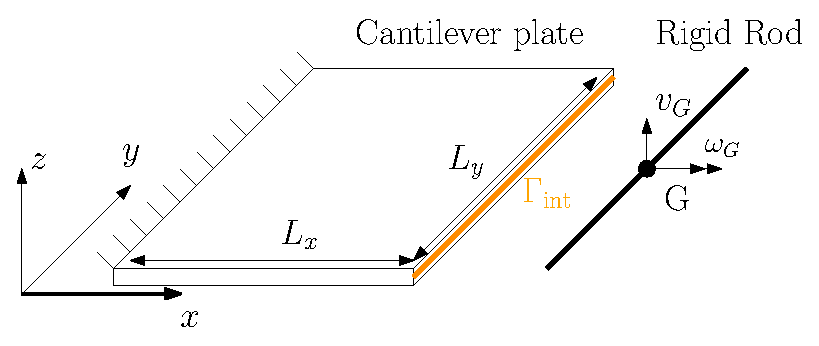
\includegraphics[height=0.25\textheight]{Figures/presentation_images_Andrea/plate_rod_separated.eps}
\end{tcolorbox}
\end{column}

\begin{column}{.43\textwidth}
\begin{tcolorbox}
	\centering
	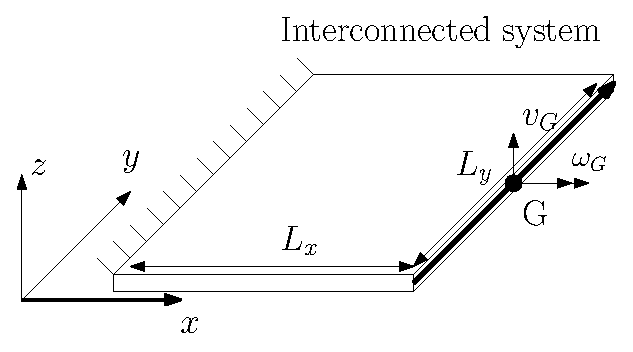
\includegraphics[height=0.25\textheight]{Figures/presentation_images_Andrea/plate_rod_welded.eps}
\end{tcolorbox}	
\end{column}
\end{columns}


\end{frame}




\begin{frame}{Boundary interconnection}
\only<1>{
	The system is composed by a cantilever plate connected to a rigid rod:
	\begin{minipage}{.4\linewidth}
		\begin{equation*}
		\text{dpH}\qquad
		\begin{aligned}
		\partial_t {\mathbf{x}}_1 &= \mathcal{J} \, \delta_{\mathbf{x}_1} {H_1}, \\
		{\mathbf{u}}_{\partial, 1}  &= \mathcal{B}_\partial \, \delta_{\mathbf{x}_1} {H_1}, \\
		{\mathbf{y}}_{\partial, 1} &= \mathcal{C}_\partial \, \delta_{\mathbf{x}_1} {H_1}, \\
		\end{aligned}
		\end{equation*}
	\end{minipage}
	\begin{minipage}{.45\linewidth}
		\begin{equation*}
		\text{pH} \qquad
		\begin{aligned}
		\dot{\mathbf{x}}_2 &= \mathbf{J} \nabla_{\mathbf{x}_2} {H_2} + \mathbf{B} \mathbf{u}_2, \\
		\mathbf{y}_{2} &= \mathbf{B}^\top \nabla_{\mathbf{x}_2} {H_2}, \\
		\end{aligned}
		\end{equation*}
	\end{minipage} %
	
	\vspace{.3cm}
	
	where $\mathbf{x}_2 \in \mathbb{R}^n, \mathbf{u}_2, \mathbf{y}_2 \in \mathbb{R}^m$ and $\mathbf{x}_1 \in {X}$,  $\mathbf{u}_{\partial, 1}  \in {U}, \, \mathbf{y}_{\partial, 1} \in  {Y} = {U}^\prime$ belong to  Hilbert spaces,  and  $\mathcal{B}_\partial: {X} \rightarrow {U}, \; \mathcal{C}_\partial: {X} \rightarrow {Y}$ are boundary operators. \\ The duality pairings for the boundary ports are denoted by
	\[
	\inner[{U}, {Y}]{\mathbf{u}_{\partial, 1}}{\mathbf{y}_{\partial, 1}},  \qquad
	\inner[\mathbb{R}^m]{\mathbf{u}_{2}}{\mathbf{y}_{2}}.
	\]
	For the interconnection, consider the compact operator $\mathcal{W}: Y \rightarrow \mathbb{R}^m$ and the following power-preserving interconnection
	\begin{equation*}
	\label{eq:int_inf}
	\mathbf{u}_2 = -\mathcal{W} \, \mathbf{y}_{\partial, 1},  \qquad \mathbf{u}_{\partial, 1} = \mathcal{W}^* \, \mathbf{y}_2.
	\end{equation*}
}

\only<2>{\vspace{.5cm}\centering 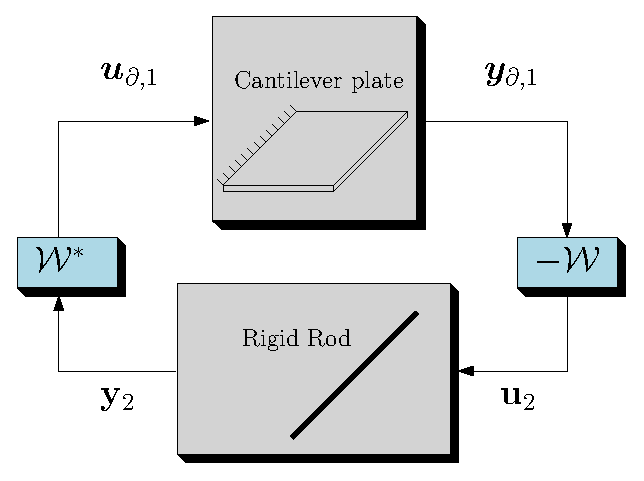
\includegraphics[width=0.6\textwidth]{Figures/presentation_images_Andrea/pp_interconnection_platerod.eps}}

\end{frame}

\begin{frame}{Kirchhoff plate welded to a rigid rod}
\begin{equation*}\small
\begin{aligned}
\text{Plate} \; (\Omega &= [0, L_x] \times [0, L_y]) \\
\begin{bmatrix}
\rho h & 0 \\ 0 & \mathcal{\bm{C}}_b \\
\end{bmatrix}
\frac{\partial}{\partial t}
\begin{bmatrix}
{e}_w \\ \mathbf{E}_\kappa \\
\end{bmatrix} &= 
\begin{bmatrix}
0 & -\div\Div \\ \nabla^2 & 0 \\
\end{bmatrix}
\begin{bmatrix}
{e}_w \\ \mathbf{E}_\kappa \\
\end{bmatrix} \\
u_{\partial, \text{pl}} &= {e}_w (x = L_x, y), \\
y_{\partial, \text{pl}} &= \widetilde{q}_n(x = L_x, y).
\end{aligned} \qquad 
\begin{aligned}
\text{Rigid rod} \\
\begin{bmatrix}
M & 0 \\
0   & J_G \\
\end{bmatrix} 
\displaystyle \frac{d}{dt}
\begin{pmatrix}
v_G \\ \omega_G \\
\end{pmatrix} & = \begin{pmatrix}
F_z \\ T_x \\
\end{pmatrix} = \mathbf{u}_{\text{rod}}\vspace{1mm}, \\
\mathbf{y}_{\text{rod}} &= \begin{pmatrix}
v_G \\ \omega_{G} \\
\end{pmatrix},
\end{aligned}
\end{equation*}
$Y$ is the space of square-integrable functions with support on $\Gamma_{\text{int}} = \left\{x=L_x\right\}$. \\
The interconnection operator  provides the total \underline{force} and \underline{torque} acting on the rigid rod
\begin{equation*}
\mathcal{W} y_{\partial, \text{pl}} =  - \begin{pmatrix}
F_z \\
T_x \\
\end{pmatrix} = \begin{pmatrix}
\int_{\Gamma_{\text{int}}} y_{\partial, \text{pl}} \dd{s} \\
\int_{\Gamma_{\text{int}}} \left( y - L_y/2 \right) y_{\partial, \text{pl}} \dd{s} \\
\end{pmatrix}.
\end{equation*}
The adjoint operator provides a rigid movement as the plate input at $\Gamma_{\text{int}}$
\begin{align*}
\left\langle \mathcal{W} y_{\partial, \text{pl}}, \; \mathbf{y}_{\text{rod}} \right\rangle_{\mathbb{R}^m} &= \left\langle y_{\partial, \text{pl}}, \, \mathcal{W}^* \mathbf{y}_{\text{rod}}\right\rangle_{L^2(\Gamma_{\text{int}})}, \\
\mathcal{W}^* \mathbf{y}_{\text{rod}} &= v_G + \omega_{G} \left( y - L_y/2 \right).
\end{align*}
\end{frame}

\frame{\frametitle{Simulation Results}
  %\begin{frame}
\begin{columns}
\begin{column}{.35\textwidth}
  \movie[start=0s, label=cells, height = 6cm, width =7cm, showcontrols=true, poster]{}{Videos/Kirchh_NoRod.ogv}
  %\end{frame}
\end{column}
\begin{column}{.55\textwidth}
\movie[start=0s, label=cells, height = 6cm, width =7cm, showcontrols=true, poster]{}{Videos/KirchhRod.ogv}
\end{column}
\end{columns}
  
}


%%%%%%%%%
\iffalse
\frame{\frametitle{Interconnected Kirchhoff plates}
%\begin{frame}
  \centering
  \movie[start=0s, label=cells, height = 7cm, width =8cm, showcontrols=true, poster]{}{Videos/Kirchh_NoRod.ogv}
 %\end{frame} 
}

\frame{\frametitle{Interconnected Kirchhoff plates}
%\begin{frame}
  \centering
  \movie[start=0s, label=cells, height = 7cm, width =8cm, showcontrols=true, poster]{}{Videos/KirchhRod.ogv}
 %\end{frame} 
}
\fi
%%%%%%%%%%%%%%%%

\frame{\frametitle{Hamiltonian behaviour}
\includegraphics[width=0.48\textwidth]{Figures/presentation_images_Andrea/HamiltonianNoRod.eps}
\includegraphics[width=0.48\textwidth]{Figures/presentation_images_Andrea/HamiltonianRod.eps}
  }

%%%%%%%%%%%%%%%%%%%% RLC
\subsection{RLC parallel circuit with Joule's effect}

\begin{frame}

\onslide<1-> 
\begin{center}
\textbf{Interconnections of several pHs.}
\end{center}

\begin{figure}[ht!]
\centering
\includegraphics[width=0.4\textwidth]{Figures/RLC-Parallel-Circuit}
\end{figure}

\onslide<2-> 
\begin{itemize}
\item \textbf{Capacitor:} $C \frac{\dd}{\dd t} U_C(t) = I_C(t)$;

If $q \eqdef C U_C$, $\frac{\dd}{\dd t} q(t) = I_C(t)$, the capacitor energy is: $\Ham_C(t) \eqdef \frac{1}{2C} q(t)^2$;
\item \textbf{Inductor:} $L \frac{\dd}{\dd t} I_L(t) = U_L(t)$;

If $\Phi \eqdef L I_L$, $\frac{\dd}{\dd t} \Phi(t) = U_L(t)$, the inductor energy is: $\Ham_L(t) \eqdef \frac{1}{2L} \Phi(t)^2$;
\item \textbf{Resistor:} its internal energy is $\U(t) \eqdef u(s(t))$.

Gibbs-Duhem relation gives: $\dd u = T \dd s$.
\end{itemize}
\onslide<3->
\begin{alertblock}{Interconnection} 
Each energy can be described as a pHs, and then interconnected thanks to comportemental laws.
\end{alertblock}

\end{frame}

\begin{frame}

\onslide<1-> 
\begin{itemize}
\item Kirchhoff laws: $I = I_C + I_L + I_R$ and $V = U_C = U_L = U_R$;
\item Ohm's law: $U_R = R I_R$;
\item Joule's effect (under Ohm's law): $dQ = U_R I_R$;
\item For the closed system, the power balance is:
\begin{center}
$
\frac{d}{dt} \green{\mc E}(t) \eqdef \frac{d}{dt} \Ham_C(t) + \frac{d}{dt} \Ham_L(t) + \frac{d}{dt} \U(t) = 0.
$
\end{center}
\end{itemize}

\vfill
\onslide<2-> 
\begin{figure}[ht!]
\centering
\includegraphics[width=0.505\textwidth]{Figures/RLC1} \; \includegraphics[width=0.475\textwidth]{Figures/RLC2}
\end{figure}

\end{frame}

%%%%%%%%%%%%%%%%%% SECTION : IMPLEMENTATION

\section{Implementation: SCRIMP software}

%%%%%%%%%%%%%%%%%%%%%%%%%%%%%%%%%%%%%%%%%%%%
\subsection{Objectives and Main features}

\begin{frame}[c]
\frametitle{{SCRIMP} software - Main objectives}


\begin{beamercolorbox}[wd=.92\paperwidth, rounded=true, shadow=true]{block body}
      


\begin{itemize}

\onslide<1->{\item To provide the INFIDHEM partners with a {\bf{state-of-the-art}}, comprehensive library for the numerical simulation of interconnected port-Hamiltonian systems (pHs).}

\onslide<1->{\item To provide well-documented tools to {\bf{make easier}} the scientific cooperation within the INFIDHEM project.}

\onslide<1->{\item To develop a software that is {\bf{easy to learn and to use}}.}  

\onslide<1->{\item To develop a software that is {\bf{easy to modify or extend}}.}


\end{itemize}
\vspace{-5mm}
  \begin{figure}[!h]
  \centering
  \includegraphics[width=3.5cm]{Figures/Logo-small.png} \\
  {\cdb{\Large{~ Simulation and ContRol of Interconnected MultiPhysical systems (SCRIMP)}}}
  \end{figure}
\end{beamercolorbox}
\end{frame}

\begin{frame}[c]
%\frametitle{{SCRIMP} software}

\begin{beamercolorbox}[wd=.92\paperwidth, rounded=true, shadow=true]{block body}
        {\bf{Programming language}}
\begin{itemize}
\onslide<1->{\item {\bf{Python}} has been selected due to its {\bf{expressivity}}, {\bf{ease of use and prototyping}} and the {\bf{availability}} of many well documented scientific libraries.}
\end{itemize}
\end{beamercolorbox}

\vskip 15pt

\begin{beamercolorbox}[wd=.92\paperwidth, rounded=true, shadow=true]{block body}
        {\bf{Interoperability}}
\begin{itemize}
\onslide<1->{\item {\bf{Python interoperability}} offers the possibility to use any external library to define a port Hamiltonian subsystem in the finite- or infinite-dimensional case.}

\onslide<1->{\item {\bf{Examples}}: simulations have been performed with PDE finite element discretizations based either on \\
  \hspace{5mm} {\bf{FEnICS}} (\url{https://fenicsproject.org/}), or\\
  \hspace{5mm} {\bf{Firedrake}} (\url{https://firedrakeproject.org/}).}

\onslide<1->{\item This seems especially important so as to tackle {\bf{coupled multi-physics}} problems, where each subsystem may correspond to a different physical phenomenon.}

\end{itemize}
\end{beamercolorbox}

\end{frame}


%%%%%%%%%%%%%%%% Classes
\subsection{Classes}


\begin{frame}[c]
\frametitle{{SCRIMP} software - Classes} %\label{lastframe}

\begin{beamercolorbox}[wd=.92\paperwidth, rounded=true, shadow=true]{block body}
        {\bf{Classes in SCRIMP are provided to}}

\begin{itemize}      

\onslide<1->{\item Define specific elementary port-Hamiltonian systems in the finite dimensional setting.}

\vspace{2ex}

\onslide<1->{\item Define how to {\bf{interconnect}} port-Hamiltonian subsystems to obtain the resulting system.} 

\vspace{2ex}


\onslide<1->{\item Represent the algebraic dynamical system as a standard {\bf{pHS}} or as a {\bf{pHDAE}} system [Beattie et al, 2018].}

\vspace{2ex}

\onslide<1->{\item Use {\bf{state-of-the-art}} numerical methods for time integration: Ongoing.}

\vspace{2ex}

\onslide<1->{\item Perform {\bf{structure-preserving}} model reduction [Gugercin et al, 2012], [Chaturantabut et al, 2016] and [Egger et al, 2018]: Ongoing.}


\end{itemize}
\end{beamercolorbox}
\end{frame}

\begin{frame}
  \frametitle{{SCRIMP} software - Classes}
\begin{beamercolorbox}[wd=.92\paperwidth, rounded=true, shadow=true]{block body}
        {\bf{Already Available Classes in SCRIMP:}}

\begin{itemize}      

\onslide<1->{\item WAVES.}

\vspace{2ex}

\onslide<1->{\item HEAT, with 3 subclasses: Lyapounov, Entropy, Energy.} 

\vspace{2ex}


\onslide<1->{\item MINDLIN PLATE.}


\end{itemize}

\vspace{2ex}
$\Longrightarrow$ More information available here:\\\\
\url{https://doi.org/10.5281/zenodo.3938600}

\end{beamercolorbox}

\vspace{2ex}

\begin{beamercolorbox}[wd=.92\paperwidth, rounded=true, shadow=true]{block body}
        {\bf{Upcoming Classes in SCRIMP:}}

\begin{itemize}      

\onslide<1->{\item KIRCHHOFF PLATE.}

\vspace{2ex}

\onslide<1->{\item MAXWELL.} 


\end{itemize}
\end{beamercolorbox}

\end{frame}


%%%%%%%%%%%%%%%%%%%%%%%%%%
\section*{Conclusions and references}

\begin{frame}{Conclusions and more}

\onslide<1->
\begin{block}{PFEM 4 PHS}
\begin{itemize}
\item \textbf{Add \textit{appropriate} ports} to get the extended structure operator;
\item Write down \textbf{weak formulations};
\item Apply \textbf{Stokes formula on a \red{P}artition} of the system;
\item Apply the \textbf{\red{F}inite \red{E}lement \red{M}ethod};
\item Take the \textbf{Constitutive Relations} into account, separately and accurately.
\end{itemize}
\end{block}
\vfill

\onslide<2->
\begin{block}{PFEM goes further}
\begin{itemize}
%\item \textbf{Mixed} boundary conditions: Lagrange multipliers;
\item Boundary (or distributed unbounded) \textbf{damping}: output feedback law;
  %\item Works for other differential operators ($\div \circ {\rm Div}$, ${\rm Grad} \circ \grad$, $\curl$, etc. thanks to \textbf{Stokes' formula} and its corollaries);
  \item Structure-preserving discretization of the divergences (DAE) in  Maxwell's equations;
  \item Structured \textbf{model reduction} for 3D Maxwell's equation;
\item \textbf{Non-linearity}: exported in the constitutive relations (DAE with higher index);
%\item And probably more!
\end{itemize}
\end{block}

\end{frame}

\begin{frame}{References (on PFEM)}

{\tiny\vspace*{-0.15cm}
\begin{itemize}
\item[\biblio] \red{A structure-preserving Partitioned Finite Element Method for the 2D wave equation}

\textbf{Cardoso-Ribeiro F.L., Matignon D., Lef\`evre L.}

\textit{IFAC-PapersOnLine, vol.51(3), pp.119--124 (2018)}, LHMNC 2018
\vfill
\item[\biblio] \blue{Partitioned Finite Element Method for port-Hamiltonian systems with Boundary Damping: Anisotropic Heterogeneous 2D wave equations}

\textbf{Serhani A., Matignon D., Haine G.}

\textit{IFAC-PapersOnLine, vol.52(2), pp.96--101 (2019)}, CPDE 2019
\vfill
\item[\biblio] \blue{Port-Hamiltonian modeling, discretization and feedback control of a circular water tank.}

\textbf{Cardoso-Ribeiro, F.L., Brugnoli, A., Matignon, Denis, Lef{\`e} vre, L.}

\textit{2019 IEEE 58th Conference on Decision and Control (CDC)}, CDC 2019
\vfill
\item[\biblio] \blue{Port-Hamiltonian formulation and symplectic discretization of plate models Part I: Mindlin model for thick plates}

\textbf{Brugnoli A., Alazard D., Pommier-Budinger V., Matignon D.}

\textit{Applied Mathematical Modelling, vol.75, pp.940--960 (2019)}
\vfill
\item[\biblio] \blue{Port-Hamiltonian formulation and symplectic discretization of plate models Part II: Kirchhoff model for thin plates}

\textbf{Brugnoli A., Alazard D., Pommier-Budinger V., Matignon D.}

\textit{Applied Mathematical Modelling, vol.75, pp.961--981 (2019)}
\vfill
\item[\biblio] \blue{Anisotropic heterogeneous n-D heat equation with boundary control and observation: I. Modeling as port-Hamiltonian system}

\textbf{Serhani A., Haine G., Matignon D.}

\textit{IFAC-PapersOnLine, vol.52(7), pp.51--56 (2019)}, TFMST 2019
\vfill
\item[\biblio] \blue{Anisotropic heterogeneous n-D heat equation with boundary control and observation: II. Structure-preserving discretization}

\textbf{Serhani A., Haine G., Matignon D.}

\textit{IFAC-PapersOnLine, vol.52(7), pp.57--62 (2019)}, TFMST 2019
\vfill
\item[\biblio] \blue{A Partitioned Finite Element Method for the Structure-Preserving Discretization of Damped Infinite-Dimensional Port-Hamiltonian Systems with Boundary Control}

\textbf{Serhani A., Matignon D., Haine G.}

\textit{Lecture Notes in Computer Science (GSI 2019), pp.549--558}
\vfill
\item[\biblio] \blue{Modelling and structure-preserving discretization of Maxwell’s equations as port-Hamiltonian system}

\textbf{Payen G.,  Matignon D., Haine G.}

\textit{IFAC-PapersOnLine, vol.53(2), pp.7671--7676 (2020)}, IFAC WC 2020
\vfill
\item[\biblio] \red{A Partitioned Finite-Element Method (PFEM) for power-preserving discretization of open systems of conservation laws}

\textbf{Cardoso-Ribeiro F.L., Matignon D., Lef\`evre L.}

\textit{IMA J. Mathematics of Control and Information, vol.00 , pp. 1--41 (2020)}


\end{itemize}}
\end{frame}


\begin{frame}{References (on PFEM)}

{\tiny\vspace*{-0.15cm}
\begin{itemize}
\item[\biblio] \blue{Numerical analysis of a structure-preserving space-discretization for an anisotropic and heterogeneous boundary controlled $N$-dimensional wave equation as port-Hamiltonian system}

\textbf{Haine G., Matignon D., Serhani A.}

\textit{{\tt https://arxiv.org/abs/2006.15032}}
%\vfill
\item[\biblio] \blue{Numerical approximation of port-Hamiltonian systems for
hyperbolic or parabolic partial differential equations}

\textbf{Brugnoli A., Haine G., Serhani A., Vasseur X.}

\textit{{\tt https://arxiv.org/abs/2007.08326}}


\end{itemize}}
\end{frame}
  
\appendix

%%%%%%%%%%%%%%%%%%%%% APPENDIX 1 :  Internal Dissipation
\section{Internal Dissipation}

\subsection{Internal Dissipation}
\begin{frame}{Internal Dissipation: Dissipative Ports}

\onslide<1-> The Hamiltonian is always the total energy:
$$
\Ham(\alp_q, \alph_p) 
\eqdef \frac{1}{2} \int_\Omega \left( \alp_q \cdot \Tens \cdot \alp_q + \frac{1}{\rhoo} \alph_p^2 \right).
$$\vfill\vspace{-2pt}
Internal dissipation $\epso (\x) \partial_t w(t,\x) = \epso (\x) \eff_p(t,\x)$ is added, with $\epso\ge0$:
$$
\left\{\begin{array}{rl}
\partial_t \alp_q &= \grad \left( \eff_p \right), \\
\partial_t \alph_p &= \div \left( \e_q \right) - \epso \eff_p,
\end{array}\right.
\qquad
\left\{\begin{array}{rll}
\u &= \eff_p, \\
\y &= \e_q \cdot \n.
\end{array}\right.
$$
\onslide<2->
$$
\matl \partial_t \alp_q \\ \partial_t \alph_p \matr 
= \matl 0 & \grad \\ \div & -\epso \matr
\matl \e_q \\ \eff_p \matr \; \leadsto \; J \eqdef \matl 0 & \grad \\ \div & 0 \matr, \quad R \eqdef \matl 0 & 0 \\ 0 & \epso \matr.
$$
\onslide<3-> Adding \textbf{dissipative ports} $\flo_r$ and $\eff_r$ and a \textbf{dissipative constitutive relation}:
$$
\underset{\blue{\boldsymbol \oplus} \; \eff_r = \epso \flo_r}{\Longrightarrow}
\qquad \matl \partial_t \alp_q \\ \partial_t \alph_p \\ \flo_r \matr 
= \matl 0 & \grad & 0 \\ \div & 0 & -I \\ 0 & I & 0 \matr
\matl \e_q \\ \eff_p \\ \eff_r \matr.
$$
\vspace{-2pt}
\onslide<4->
\begin{alertblock}{Lossy \textbf{Power Balance}}
\centering
$
\dsp \frac{\rm d}{{\rm d}t}\Ham (\alp_q, \alph_p) 
= - \psl \epso \eff_p, \eff_p \psr_{L^2} + \psl \y, \u \psr_{H^{-\frac{1}{2}},H^{\frac{1}{2}}} \; \le \; \psl \y, \u \psr_{H^{-\frac{1}{2}},H^{\frac{1}{2}}}.
$
\end{alertblock}

\end{frame}

\begin{frame}{Internal Dissipation: PFEM}

\onslide<1-> Approximating $\flo_r$ and $\eff_r$ in the FEM basis ${\boldsymbol \phi}_p$, PFEM gives:
$$
\underbrace
{\matl
\vector{M}_q & 0 & 0 & 0 \\
0 & M_p & 0 & 0 \\
0 & 0 & M_p & 0 \\
0 & 0 & 0 & M_\partial 
\matr}_{{\mc M}}
\underbrace
{\matl
\frac{\rm d}{{\rm d}t}\underline{\alph}_q(t) \\
\frac{\rm d}{{\rm d}t}\underline{\alph}_p(t) \\
\underline{\flo}_r(t) \\
- \underline{\y}(t) 
\matr}_{\f_d}
=
\underbrace
{\matl
0 & D & 0 & B \\
-D^\top & 0 & M_p & 0 \\
0 & -M_p & 0 & 0 \\
-B^\top & 0 & 0 & 0 
\matr}_{\J_d}
\underbrace
{\matl
\underline{\eff}_q(t) \\
\underline{\eff}_p(t) \\
\underline{\eff}_r(t) \\
\underline{\u}(t) 
\matr}_{\e_d}.
$$
\onslide<2-> The \textbf{dissipative constitutive relation} is discretized as: \\
\centering
$
M_p \cdot \underline{\eff}_r = \Eo \cdot \underline{\flo}_r, \qquad \qquad
$
with
$
\Eo \eqdef \int_\Omega \epso {\boldsymbol \phi}_p \cdot {\boldsymbol \phi}_p^\top \ge 0.
$
\onslide<3-> 
\begin{alertblock}{Discrete Lossy \textbf{Power Balance}}
\centering
$
\frac{\rm d}{{\rm d}t}\Ham_d \left( \underline{\alph}_q, \underline{\alph}_p \right) = - \underline{\eff}_p^\top \cdot \Eo \cdot \underline{\eff}_p + \underline{\u}^\top \cdot M_\partial \cdot \underline{\y} \; \le \; \underline{\u}^\top \cdot M_\partial \cdot \underline{\y}.
$
\end{alertblock}
\vfill
\warning In practice, $\flo_r$ and $\eff_r$ do not need to be discretized in the basis of $\flo_p$ and $\eff_p$.

\end{frame}

%%%%%%%%%%%%%%%%%%%%%%%%%%%% APPENDIX 2 : ENTROPY
\section{Entropy}

\begin{frame}{Accretion: Entropy}

\onslide<1-> 
\begin{block}{Hamiltonian: Entropy}
\centering
$
\dsp \S(\rhoo(\x) u(t,\x)) \eqdef \int_\Omega \rhoo(\x) s(\rhoo(\x) u(t,\x)) \dd \x,
$
\flushleft \emph{Energy variable} : $\alph_u \eqdef \rhoo u$, \emph{co-energy variable} : $\eff_u \eqdef \delta_{\alph_u} \S = \beta$.
\end{block}
\vfill
\onslide<2-> 
\begin{alertblock}{\textbf{Power Balance} (second law of thermodynamics)}
\centering
$
\dsp \frac{\rm d}{{\rm d}t}\S = \int_{\Omega} \sigma - \psl \vector{J}_Q \cdot \n, \beta \psr_{H^{-\frac{1}{2}},H^{\frac{1}{2}}}.
$\vfill 
\end{alertblock}
\vfill
\onslide<3-> 
Defining $\flo_u \eqdef \partial_t \alph_u = \rhoo \partial_t u$, $\eff_u = \beta$, $\f_Q \eqdef -\grad \left( \beta \right)$, and $\e_Q \eqdef \vector{J}_Q$
$$
\matl \flo_u \\ \f_Q \matr = \matl 0 & -\div \\ -\grad & 0 \matr \matl \eff_u \\ \e_Q \matr.
$$

\end{frame}

\begin{frame}{Accretion: Entropy}

\onslide<1-> 
At least two choices for \blue{boundary control}: $\eff_u$ or $\e_Q \cdot \n$.\vfill
With \blue{\textit{inward} heat flux} $\nuo = -\e_Q \cdot \n$, the output is $\y = \eff_u$, \ie the \red{boundary reciprocal temperature}, and the discretized system is:
$$
\matl
M & 0 & 0 \\
0 & \vector{M} & 0 \\
0 & 0 & M_\partial 
\matr
\matl
\underline{\flo}_u \\
\underline{\flo}_Q \\
-\underline{\y}
\matr
=
\matl
0 & \widetilde D & \widetilde B \\
-\widetilde D^\top & 0 & 0 \\
-\widetilde B^\top & 0 & 0
\matr
\matl
\underline{\eff}_u \\
\underline{\eff}_Q \\
\underline{\nuo}
\matr.
$$
\onslide<2-> 
\textbf{\textit{Non-linear} constitutive relations} from: \hfill $\rhoo C_V = \alph_u \eff_u$ \hfill \& \hfill $\eff_u^2 \vector{\eff}_Q = - \Tens \cdot \vector{\flo}_Q$.\vfill
\onslide<3-> 
\begin{alertblock}{Accretive \textbf{Power Balance} (second law of thermodynamics)}
\centering
$
\dsp \frac{\rm d}{{\rm d}t}\S = - \int_\Omega \f_Q \cdot \e_Q + \psl \nuo, \y \psr_{H^{-\frac{1}{2}},H^{\frac{1}{2}}} \; \ge \; \psl \nuo, \y \psr_{H^{-\frac{1}{2}},H^{\frac{1}{2}}}.
$
\end{alertblock}
\onslide<4-> 
\begin{alertblock}{Discrete accretive \textbf{Power Balance} (second law of thermodynamics)}
\centering
$
\dsp \frac{\rm d}{{\rm d}t}\S = - \underline{\flo}_Q \cdot \vector{M} \cdot \underline{\eff}_Q + \underline{\nuo}^\top \cdot M_\partial \cdot \underline{\y} \; \ge \; \underline{\nuo}^\top \cdot M_\partial \cdot \underline{\y}.
$
\end{alertblock}

\end{frame}


\iffalse
%%%%%%%%%%%%%%%%%%%%%%%%%%%% APPENDIX 3 : Stokes Dirac
\section{Stokes-Dirac structure}

\begin{frame}{Associated (Stokes-)Dirac structures}

\begin{itemize}
\item<1->
The \emph{effort space} $\E$ (Hilbert space) and $\e \eqdef \matl \e_{\alp}, & \e_R, & \u \matr^\top$;
\item<2->
The \emph{flow space} $\F \eqdef \E'$ and $\f \eqdef \matl \partial_t \alp, & \f_R, & - \y \matr^\top$;
\item<3->
The \emph{\textit{extended structure} operator} $\J \eqdef \matl J & -I & B \\ I & 0 & 0 \\ - B^* & 0 & 0 \matr$;
\item<4->
The \emph{Bond space} $\mc B \eqdef \F \times \E$, with symmetrized bilinear product:
$$
\pbl \matl \f^1 \\ \e^1 \matr, \matl \f^2 \\ \e^2 \matr \pbr_{\mc B} \eqdef \psl \f^1, \e^2 \psr_{\F, \E} + \psl \f^2, \e^1 \psr_{\F, \E};
$$
\item<5->
The \emph{Dirac structure} $\D \eqdef \graph \left( \J \right) \subset \mc B$, \ie $\D^{[\perp]} = \D$ with:
$$
\mc D^{[\perp]} \eqdef \left\{ \matl \f \\ \e \matr \in \mc B \; \Biggm| \; \pbl \matl \f \\ \e \matr, \matl \widetilde \f \\ \widetilde \e \matr \pbr_{\mc B} = 0, \; \Forall \matl \widetilde \f \\ \widetilde \e \matr \in \mc D \right\}.
$$
\item<6->
The \emph{dissipative constitutive relation} $\e_R = R \f_R$;
\end{itemize}
\onslide<5-> \warning Hypotheses on $J$ and $B$ are needed for $\D$ to be a (Stokes-)Dirac structure!

\end{frame}

\begin{frame}{Resulting Differential Algebraic Equations (DAE)}

\onslide<1-> 
\begin{tcolorbox}
$
\psl \f(t), \e(t) \psr_{\F, \E} 
= 0, \Forall \matl \f(t), \e(t) \matr \in \D, \Forall t \ge 0.
$
\end{tcolorbox}
\vfill
\onslide<2-> Let $\left( \partial_t \alp, \f_R, -\y, \e_{\alp}, \e_R, \u \right)^\top$ be in $\D$. \\
Adding $\e_R = R \f_R$: \red{\textbf{the lossy power balance is satisfied}}!
\vfill
\onslide<3->
\begin{tcolorbox}
$\red{\Longrightarrow}$ Flow/effort representation \red{generalizes} the above state representation with $J-R$, \blue{\it and PFEM appears to be very well-suited to it!}
\vfill
\centering PHS + DAE = \red{\bf PHDAE}.
\end{tcolorbox}
\vfill
\onslide<4->
\begin{alertblock}{Main result}
PFEM gives rise to a \textbf{finite-dimensional Dirac structure} \textit{\red{containing}} a \emph{discrete version of the (lossy) power balance} for the \emph{discrete Hamiltonian}.
\end{alertblock}

\end{frame}
\fi

\end{document}
